% Options for packages loaded elsewhere
\PassOptionsToPackage{unicode}{hyperref}
\PassOptionsToPackage{hyphens}{url}
%
\documentclass[
  ignorenonframetext,
]{beamer}
\usepackage{pgfpages}
\setbeamertemplate{caption}[numbered]
\setbeamertemplate{caption label separator}{: }
\setbeamercolor{caption name}{fg=normal text.fg}
\beamertemplatenavigationsymbolsempty
% Prevent slide breaks in the middle of a paragraph
\widowpenalties 1 10000
\raggedbottom
\setbeamertemplate{part page}{
  \centering
  \begin{beamercolorbox}[sep=16pt,center]{part title}
    \usebeamerfont{part title}\insertpart\par
  \end{beamercolorbox}
}
\setbeamertemplate{section page}{
  \centering
  \begin{beamercolorbox}[sep=12pt,center]{part title}
    \usebeamerfont{section title}\insertsection\par
  \end{beamercolorbox}
}
\setbeamertemplate{subsection page}{
  \centering
  \begin{beamercolorbox}[sep=8pt,center]{part title}
    \usebeamerfont{subsection title}\insertsubsection\par
  \end{beamercolorbox}
}
\AtBeginPart{
  \frame{\partpage}
}
\AtBeginSection{
  \ifbibliography
  \else
    \frame{\sectionpage}
  \fi
}
\AtBeginSubsection{
  \frame{\subsectionpage}
}
\usepackage{amsmath,amssymb}
\usepackage{iftex}
\ifPDFTeX
  \usepackage[T1]{fontenc}
  \usepackage[utf8]{inputenc}
  \usepackage{textcomp} % provide euro and other symbols
\else % if luatex or xetex
  \usepackage{unicode-math} % this also loads fontspec
  \defaultfontfeatures{Scale=MatchLowercase}
  \defaultfontfeatures[\rmfamily]{Ligatures=TeX,Scale=1}
\fi
\usepackage{lmodern}
\usetheme[]{Madrid}
\ifPDFTeX\else
  % xetex/luatex font selection
\fi
% Use upquote if available, for straight quotes in verbatim environments
\IfFileExists{upquote.sty}{\usepackage{upquote}}{}
\IfFileExists{microtype.sty}{% use microtype if available
  \usepackage[]{microtype}
  \UseMicrotypeSet[protrusion]{basicmath} % disable protrusion for tt fonts
}{}
\makeatletter
\@ifundefined{KOMAClassName}{% if non-KOMA class
  \IfFileExists{parskip.sty}{%
    \usepackage{parskip}
  }{% else
    \setlength{\parindent}{0pt}
    \setlength{\parskip}{6pt plus 2pt minus 1pt}}
}{% if KOMA class
  \KOMAoptions{parskip=half}}
\makeatother
\usepackage{xcolor}
\newif\ifbibliography
\usepackage{color}
\usepackage{fancyvrb}
\newcommand{\VerbBar}{|}
\newcommand{\VERB}{\Verb[commandchars=\\\{\}]}
\DefineVerbatimEnvironment{Highlighting}{Verbatim}{commandchars=\\\{\}}
% Add ',fontsize=\small' for more characters per line
\usepackage{framed}
\definecolor{shadecolor}{RGB}{248,248,248}
\newenvironment{Shaded}{\begin{snugshade}}{\end{snugshade}}
\newcommand{\AlertTok}[1]{\textcolor[rgb]{0.94,0.16,0.16}{#1}}
\newcommand{\AnnotationTok}[1]{\textcolor[rgb]{0.56,0.35,0.01}{\textbf{\textit{#1}}}}
\newcommand{\AttributeTok}[1]{\textcolor[rgb]{0.13,0.29,0.53}{#1}}
\newcommand{\BaseNTok}[1]{\textcolor[rgb]{0.00,0.00,0.81}{#1}}
\newcommand{\BuiltInTok}[1]{#1}
\newcommand{\CharTok}[1]{\textcolor[rgb]{0.31,0.60,0.02}{#1}}
\newcommand{\CommentTok}[1]{\textcolor[rgb]{0.56,0.35,0.01}{\textit{#1}}}
\newcommand{\CommentVarTok}[1]{\textcolor[rgb]{0.56,0.35,0.01}{\textbf{\textit{#1}}}}
\newcommand{\ConstantTok}[1]{\textcolor[rgb]{0.56,0.35,0.01}{#1}}
\newcommand{\ControlFlowTok}[1]{\textcolor[rgb]{0.13,0.29,0.53}{\textbf{#1}}}
\newcommand{\DataTypeTok}[1]{\textcolor[rgb]{0.13,0.29,0.53}{#1}}
\newcommand{\DecValTok}[1]{\textcolor[rgb]{0.00,0.00,0.81}{#1}}
\newcommand{\DocumentationTok}[1]{\textcolor[rgb]{0.56,0.35,0.01}{\textbf{\textit{#1}}}}
\newcommand{\ErrorTok}[1]{\textcolor[rgb]{0.64,0.00,0.00}{\textbf{#1}}}
\newcommand{\ExtensionTok}[1]{#1}
\newcommand{\FloatTok}[1]{\textcolor[rgb]{0.00,0.00,0.81}{#1}}
\newcommand{\FunctionTok}[1]{\textcolor[rgb]{0.13,0.29,0.53}{\textbf{#1}}}
\newcommand{\ImportTok}[1]{#1}
\newcommand{\InformationTok}[1]{\textcolor[rgb]{0.56,0.35,0.01}{\textbf{\textit{#1}}}}
\newcommand{\KeywordTok}[1]{\textcolor[rgb]{0.13,0.29,0.53}{\textbf{#1}}}
\newcommand{\NormalTok}[1]{#1}
\newcommand{\OperatorTok}[1]{\textcolor[rgb]{0.81,0.36,0.00}{\textbf{#1}}}
\newcommand{\OtherTok}[1]{\textcolor[rgb]{0.56,0.35,0.01}{#1}}
\newcommand{\PreprocessorTok}[1]{\textcolor[rgb]{0.56,0.35,0.01}{\textit{#1}}}
\newcommand{\RegionMarkerTok}[1]{#1}
\newcommand{\SpecialCharTok}[1]{\textcolor[rgb]{0.81,0.36,0.00}{\textbf{#1}}}
\newcommand{\SpecialStringTok}[1]{\textcolor[rgb]{0.31,0.60,0.02}{#1}}
\newcommand{\StringTok}[1]{\textcolor[rgb]{0.31,0.60,0.02}{#1}}
\newcommand{\VariableTok}[1]{\textcolor[rgb]{0.00,0.00,0.00}{#1}}
\newcommand{\VerbatimStringTok}[1]{\textcolor[rgb]{0.31,0.60,0.02}{#1}}
\newcommand{\WarningTok}[1]{\textcolor[rgb]{0.56,0.35,0.01}{\textbf{\textit{#1}}}}
\usepackage{graphicx}
\makeatletter
\def\maxwidth{\ifdim\Gin@nat@width>\linewidth\linewidth\else\Gin@nat@width\fi}
\def\maxheight{\ifdim\Gin@nat@height>\textheight\textheight\else\Gin@nat@height\fi}
\makeatother
% Scale images if necessary, so that they will not overflow the page
% margins by default, and it is still possible to overwrite the defaults
% using explicit options in \includegraphics[width, height, ...]{}
\setkeys{Gin}{width=\maxwidth,height=\maxheight,keepaspectratio}
% Set default figure placement to htbp
\makeatletter
\def\fps@figure{htbp}
\makeatother
\setlength{\emergencystretch}{3em} % prevent overfull lines
\providecommand{\tightlist}{%
  \setlength{\itemsep}{0pt}\setlength{\parskip}{0pt}}
\setcounter{secnumdepth}{-\maxdimen} % remove section numbering
\logo{
\includegraphics[height=1cm,width=3cm]{logo.png}}
\usetheme{Madrid}
\usefonttheme{serif}
\setbeamertemplate{navigation symbols}{}
\usepackage{lmodern}  % for bold teletype font
\usepackage{amsmath}  % for \hookrightarrow
\usepackage{xcolor}   % for \textcolor


\ifLuaTeX
  \usepackage{selnolig}  % disable illegal ligatures
\fi
\IfFileExists{bookmark.sty}{\usepackage{bookmark}}{\usepackage{hyperref}}
\IfFileExists{xurl.sty}{\usepackage{xurl}}{} % add URL line breaks if available
\urlstyle{same}
\hypersetup{
  pdftitle={Leksioni 10},
  pdfauthor={Endri Raco},
  hidelinks,
  pdfcreator={LaTeX via pandoc}}

\title{Leksioni 10}
\author{Endri Raco}
\date{06 May, 2024}

\begin{document}
\frame{\titlepage}

\begin{frame}[allowframebreaks]
  \tableofcontents[hideallsubsections]
\end{frame}
\hypertarget{parashikimi-i-tarifuxebs-suxeb-taksive-nuxeb-new-york-city}{%
\section{Parashikimi i Tarifës së Taksive në New York
City}\label{parashikimi-i-tarifuxebs-suxeb-taksive-nuxeb-new-york-city}}

\begin{frame}[fragile]{Leximi i të dhënave dhe eksplorimi i parë}
\protect\hypertarget{leximi-i-tuxeb-dhuxebnave-dhe-eksplorimi-i-paruxeb}{}
\AddToHookNext{env/Highlighting/begin}{\tiny}

\begin{Shaded}
\begin{Highlighting}[]
\CommentTok{\# ngarkoni disa module të parazgjedhura të Python}
\ImportTok{import}\NormalTok{ numpy }\ImportTok{as}\NormalTok{ np}
\ImportTok{import}\NormalTok{ pandas }\ImportTok{as}\NormalTok{ pd}
\ImportTok{import}\NormalTok{ matplotlib.pyplot }\ImportTok{as}\NormalTok{ plt}
\ImportTok{import}\NormalTok{ seaborn }\ImportTok{as}\NormalTok{ sns}

\CommentTok{\# List available styles and choose an available one}
\BuiltInTok{print}\NormalTok{(plt.style.available)}
\NormalTok{plt.style.use(}\StringTok{"seaborn{-}v0\_8{-}whitegrid"}\NormalTok{)}

\OperatorTok{\%}\NormalTok{matplotlib inline}
\end{Highlighting}
\end{Shaded}
\end{frame}

\begin{frame}{Leximi i të dhënave dhe eksplorimi i parë}
\protect\hypertarget{leximi-i-tuxeb-dhuxebnave-dhe-eksplorimi-i-paruxeb-1}{}
\begin{itemize}
\item
  Si një dataset i madh, leximi i të gjitha të dhënave do të kërkonte
  shumë memorie.
\item
  Prandaj lexojmë një numër të kufizuar rreshtash dhe eksplorojmë të
  dhënat.
\end{itemize}
\end{frame}

\begin{frame}[fragile]{Leximi i të dhënave dhe eksplorimi i parë}
\protect\hypertarget{leximi-i-tuxeb-dhuxebnave-dhe-eksplorimi-i-paruxeb-2}{}
\AddToHookNext{env/Highlighting/begin}{\tiny}

\begin{Shaded}
\begin{Highlighting}[]
\CommentTok{\# lexoni të dhënat në kuadrin e të dhënave të pandas}
\NormalTok{df\_train }\OperatorTok{=}\NormalTok{ pd.read\_csv(}\StringTok{\textquotesingle{}data/newyork/train.csv\textquotesingle{}}\NormalTok{, nrows}\OperatorTok{=}\DecValTok{2\_000\_000}\NormalTok{, parse\_dates}\OperatorTok{=}\NormalTok{[}\StringTok{"pickup\_datetime"}\NormalTok{])}

\CommentTok{\# listoni rreshtat e parë (pikë të dhënash)}
\NormalTok{df\_train.head()}
\end{Highlighting}
\end{Shaded}
\end{frame}

\begin{frame}{Leximi i të dhënave dhe eksplorimi i parë}
\protect\hypertarget{leximi-i-tuxeb-dhuxebnave-dhe-eksplorimi-i-paruxeb-3}{}
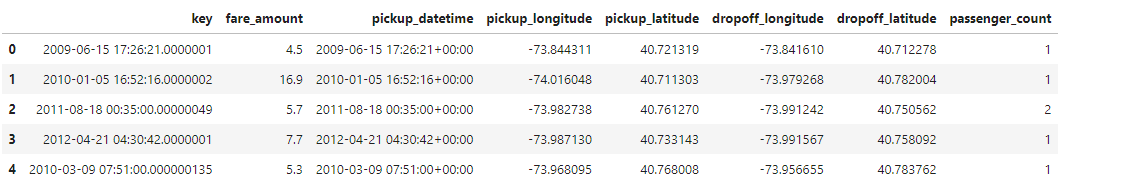
\includegraphics{./Figs/train.png}
\end{frame}

\begin{frame}[fragile]{Leximi i të dhënave dhe eksplorimi i parë}
\protect\hypertarget{leximi-i-tuxeb-dhuxebnave-dhe-eksplorimi-i-paruxeb-4}{}
\AddToHookNext{env/Highlighting/begin}{\tiny}

\begin{Shaded}
\begin{Highlighting}[]
\CommentTok{\# kontrolloni llojet e të dhënave}
\NormalTok{df\_train.dtypes}
\end{Highlighting}
\end{Shaded}
\end{frame}

\begin{frame}{Leximi i të dhënave dhe eksplorimi i parë}
\protect\hypertarget{leximi-i-tuxeb-dhuxebnave-dhe-eksplorimi-i-paruxeb-5}{}
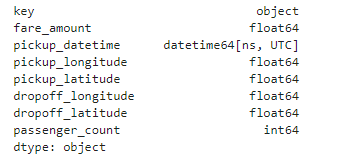
\includegraphics{./Figs/train1.png}
\end{frame}

\begin{frame}[fragile]{Leximi i të dhënave dhe eksplorimi i parë}
\protect\hypertarget{leximi-i-tuxeb-dhuxebnave-dhe-eksplorimi-i-paruxeb-6}{}
\AddToHookNext{env/Highlighting/begin}{\tiny}

\begin{Shaded}
\begin{Highlighting}[]
\CommentTok{\# kontrolloni statistikat e veçorive}
\NormalTok{df\_train.describe()}
\end{Highlighting}
\end{Shaded}
\end{frame}

\begin{frame}{Leximi i të dhënave dhe eksplorimi i parë}
\protect\hypertarget{leximi-i-tuxeb-dhuxebnave-dhe-eksplorimi-i-paruxeb-7}{}
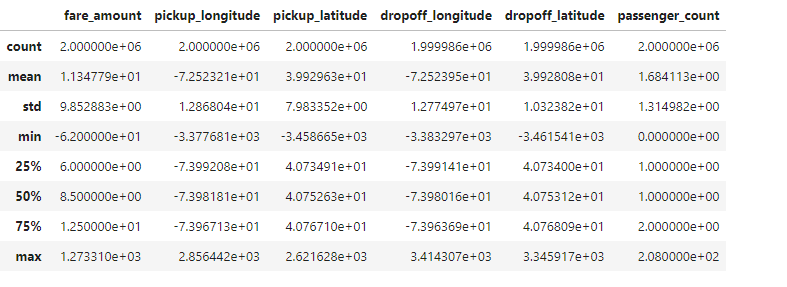
\includegraphics{./Figs/train2.png}
\end{frame}

\begin{frame}{Leximi i të dhënave dhe eksplorimi i parë}
\protect\hypertarget{leximi-i-tuxeb-dhuxebnave-dhe-eksplorimi-i-paruxeb-8}{}
Pikat e mëposhtme bien në sy:

\begin{itemize}
\item
  Tarifa minimale është negative.
\item
  Kjo nuk duket të jetë realiste, kështu që do t'i heqim nga seti i të
  dhënave.
\end{itemize}
\end{frame}

\begin{frame}{Leximi i të dhënave dhe eksplorimi i parë}
\protect\hypertarget{leximi-i-tuxeb-dhuxebnave-dhe-eksplorimi-i-paruxeb-9}{}
\begin{itemize}
\item
  Disa nga koordinatat minimale dhe maksimale të gjerësisë/gjatësisë
  janë shumë të largëta, kështu që do t'i heqim ato gjithashtu.
\item
  Tarifa mesatare është rreth 11.4 USD me një devijim standard prej 9.9
  USD.
\end{itemize}
\end{frame}

\begin{frame}[fragile]{Leximi i të dhënave dhe eksplorimi i parë}
\protect\hypertarget{leximi-i-tuxeb-dhuxebnave-dhe-eksplorimi-i-paruxeb-10}{}
\AddToHookNext{env/Highlighting/begin}{\tiny}

\begin{Shaded}
\begin{Highlighting}[]
\BuiltInTok{print}\NormalTok{(}\StringTok{\textquotesingle{}Madhësia e vjetër: }\SpecialCharTok{\%d}\StringTok{\textquotesingle{}} \OperatorTok{\%} \BuiltInTok{len}\NormalTok{(df\_train))}
\NormalTok{df\_train }\OperatorTok{=}\NormalTok{ df\_train[df\_train.fare\_amount }\OperatorTok{\textgreater{}=} \DecValTok{0}\NormalTok{]}
\BuiltInTok{print}\NormalTok{(}\StringTok{\textquotesingle{}Madhësia e re: }\SpecialCharTok{\%d}\StringTok{\textquotesingle{}} \OperatorTok{\%} \BuiltInTok{len}\NormalTok{(df\_train))}
\end{Highlighting}
\end{Shaded}
\end{frame}

\begin{frame}{Leximi i të dhënave dhe eksplorimi i parë}
\protect\hypertarget{leximi-i-tuxeb-dhuxebnave-dhe-eksplorimi-i-paruxeb-11}{}

\includegraphics{./Figs/train3.png}
\end{frame}

\begin{frame}[fragile]{Leximi i të dhënave dhe eksplorimi i parë}
\protect\hypertarget{leximi-i-tuxeb-dhuxebnave-dhe-eksplorimi-i-paruxeb-12}{}
\AddToHookNext{env/Highlighting/begin}{\tiny}

\begin{Shaded}
\begin{Highlighting}[]
\CommentTok{\# grafiku i histogramit të tarifës}
\NormalTok{df\_train[df\_train.fare\_amount }\OperatorTok{\textless{}} \DecValTok{100}\NormalTok{].fare\_amount.hist(bins}\OperatorTok{=}\DecValTok{100}\NormalTok{, figsize}\OperatorTok{=}\NormalTok{(}\DecValTok{14}\NormalTok{,}\DecValTok{3}\NormalTok{))}
\NormalTok{plt.xlabel(}\StringTok{\textquotesingle{}tarifa $USD\textquotesingle{}}\NormalTok{)}
\NormalTok{plt.title(}\StringTok{\textquotesingle{}Histogram\textquotesingle{}}\NormalTok{)}
\NormalTok{plt.show()}
\end{Highlighting}
\end{Shaded}
\end{frame}

\begin{frame}{Leximi i të dhënave dhe eksplorimi i parë}
\protect\hypertarget{leximi-i-tuxeb-dhuxebnave-dhe-eksplorimi-i-paruxeb-13}{}
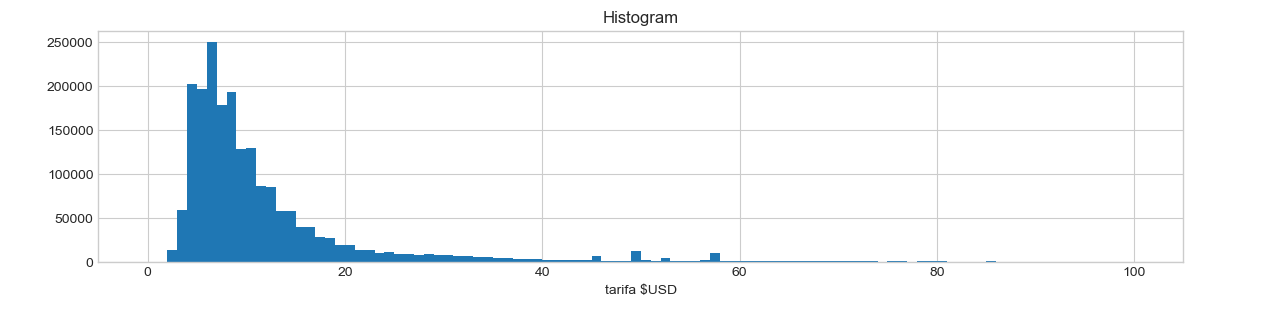
\includegraphics{./Figs/train4.png}
\end{frame}

\begin{frame}{Leximi i të dhënave dhe eksplorimi i parë}
\protect\hypertarget{leximi-i-tuxeb-dhuxebnave-dhe-eksplorimi-i-paruxeb-14}{}
\begin{itemize}
\item
  Në histogramin e \textbf{fare\_amount} ka disa pika të vogla midis 40
  dhe 60 dollarë.
\item
  Kjo mund të tregojë një çmim fiks të tarifës (p.sh. për/nga
  aeroporti).
\item
  Kjo do të eksplorohet më tej më poshtë
\end{itemize}
\end{frame}

\begin{frame}{Pastrimi i të dhënave}
\protect\hypertarget{pastrimi-i-tuxeb-dhuxebnave}{}
Fillimisht kontrollojmë për të dhëna të munguar dhe heqim rreshtat me
mungesë të dhënash për të pasur një dataset të pastër për analizë.
\end{frame}

\begin{frame}[fragile]{Pastrimi i të dhënave}
\protect\hypertarget{pastrimi-i-tuxeb-dhuxebnave-1}{}
\AddToHookNext{env/Highlighting/begin}{\tiny}

\begin{Shaded}
\begin{Highlighting}[]
\CommentTok{\# Kontrollo për të dhëna të munguar}
\BuiltInTok{print}\NormalTok{(df\_train.isnull().}\BuiltInTok{sum}\NormalTok{())}
\end{Highlighting}
\end{Shaded}
\end{frame}

\begin{frame}{Pastrimi i të dhënave}
\protect\hypertarget{pastrimi-i-tuxeb-dhuxebnave-2}{}
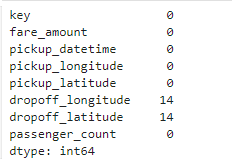
\includegraphics{./Figs/train5.png}
\end{frame}

\begin{frame}[fragile]{Pastrimi i të dhënave}
\protect\hypertarget{pastrimi-i-tuxeb-dhuxebnave-3}{}
\AddToHookNext{env/Highlighting/begin}{\tiny}

\begin{Shaded}
\begin{Highlighting}[]
\CommentTok{\# Shfaq numrin e rreshtave të vjetra dhe pastroni datasetin nga të dhënat e munguar}
\BuiltInTok{print}\NormalTok{(}\StringTok{\textquotesingle{}Numri i rreshtave të vjetra: }\SpecialCharTok{\%d}\StringTok{\textquotesingle{}} \OperatorTok{\%} \BuiltInTok{len}\NormalTok{(df\_train))}
\NormalTok{df\_train }\OperatorTok{=}\NormalTok{ df\_train.dropna(how }\OperatorTok{=} \StringTok{\textquotesingle{}any\textquotesingle{}}\NormalTok{, axis }\OperatorTok{=} \StringTok{\textquotesingle{}rows\textquotesingle{}}\NormalTok{)}
\BuiltInTok{print}\NormalTok{(}\StringTok{\textquotesingle{}Numri i rreshtave të reja: }\SpecialCharTok{\%d}\StringTok{\textquotesingle{}} \OperatorTok{\%} \BuiltInTok{len}\NormalTok{(df\_train))}
\end{Highlighting}
\end{Shaded}
\end{frame}

\begin{frame}{Pastrimi i të dhënave}
\protect\hypertarget{pastrimi-i-tuxeb-dhuxebnave-4}{}
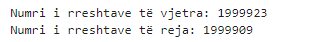
\includegraphics{./Figs/train6.png}
\end{frame}

\begin{frame}[fragile]{Të dhënat e testimit}
\protect\hypertarget{tuxeb-dhuxebnat-e-testimit}{}
Të dhënat e testimit ngarkohen për të krahasuar statistikat me datasetin
e trajnimit.

\AddToHookNext{env/Highlighting/begin}{\tiny}

\begin{Shaded}
\begin{Highlighting}[]
\CommentTok{\# Lexoni të dhënat e testimit}
\NormalTok{df\_test }\OperatorTok{=}\NormalTok{ pd.read\_csv(}\StringTok{\textquotesingle{}data/newyork/test.csv\textquotesingle{}}\NormalTok{)}
\NormalTok{df\_test.head(}\DecValTok{5}\NormalTok{)}
\end{Highlighting}
\end{Shaded}
\end{frame}

\begin{frame}{Të dhënat e testimit}
\protect\hypertarget{tuxeb-dhuxebnat-e-testimit-1}{}
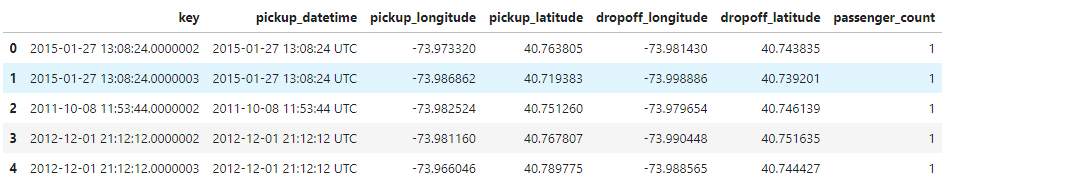
\includegraphics{./Figs/train7.png}
\end{frame}

\begin{frame}[fragile]{Statistikat e datasetit të testimit}
\protect\hypertarget{statistikat-e-datasetit-tuxeb-testimit}{}
\AddToHookNext{env/Highlighting/begin}{\tiny}

\begin{Shaded}
\begin{Highlighting}[]
\NormalTok{df\_test.describe()}
\end{Highlighting}
\end{Shaded}
\end{frame}

\begin{frame}{Statistikat e datasetit të testimit}
\protect\hypertarget{statistikat-e-datasetit-tuxeb-testimit-1}{}
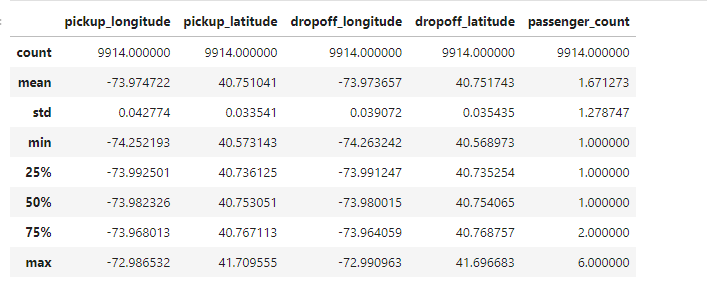
\includegraphics{./Figs/train8.png}
\end{frame}

\begin{frame}{Lokacionet}
\protect\hypertarget{lokacionet}{}
\begin{itemize}
\item
  Duke qenë se kemi të bëjmë me të dhënat e vendndodhjes, duam të
  shfaqim koordinatat në një hartë.
\item
  Kjo jep një pamje më të mirë të të dhënave.
\end{itemize}
\end{frame}

\begin{frame}{Lokacionet}
\protect\hypertarget{lokacionet-1}{}
Koordinatat e qytetit të Nju Jorkut janë
(\url{https://www.travelmath.com/cities/New+York,+NY}):

\begin{itemize}
\item
  longitude = -74.0063889
\item
  lattitude = 40.7141667
\end{itemize}
\end{frame}

\begin{frame}{Lokacionet}
\protect\hypertarget{lokacionet-2}{}
\begin{itemize}
\tightlist
\item
  Përcaktojmë një kuti kufizuese nga {[}long\_min, long\_max, latt\_min,
  latt\_max{]} duke përdorur koordinatat minimale dhe maksimale nga të
  dhënaat \textbf{test}.
\end{itemize}
\end{frame}

\begin{frame}{Lokacionet}
\protect\hypertarget{lokacionet-3}{}
\begin{itemize}
\item
  Në këtë mënyrë, sigurohemi se do trajnojmë një model për gamën e plotë
  të koordinatave
\item
  Nga Open Street Map marrim një hartë dhe fshijmë çdo pikë të dhënash
  jashtë kësaj kutie.
\end{itemize}
\end{frame}

\begin{frame}[fragile]{Lokacionet}
\protect\hypertarget{lokacionet-4}{}
\AddToHookNext{env/Highlighting/begin}{\tiny}

\begin{Shaded}
\begin{Highlighting}[]
\CommentTok{\# Koordinatat e minimumit dhe maksimumit për longitude dhe latitude në setin e testimit}
\BuiltInTok{min}\NormalTok{(df\_test.pickup\_longitude.}\BuiltInTok{min}\NormalTok{(), df\_test.dropoff\_longitude.}\BuiltInTok{min}\NormalTok{()), }\OperatorTok{\textbackslash{}}
\BuiltInTok{max}\NormalTok{(df\_test.pickup\_longitude.}\BuiltInTok{max}\NormalTok{(), df\_test.dropoff\_longitude.}\BuiltInTok{max}\NormalTok{())}
\end{Highlighting}
\end{Shaded}
\end{frame}

\begin{frame}[fragile]{Lokacionet}
\protect\hypertarget{lokacionet-5}{}
\AddToHookNext{env/Highlighting/begin}{\tiny}

\begin{Shaded}
\begin{Highlighting}[]
\ImportTok{import}\NormalTok{ ssl}
\ImportTok{import}\NormalTok{ urllib.request}
\ImportTok{from}\NormalTok{ PIL }\ImportTok{import}\NormalTok{ Image}
\ImportTok{import}\NormalTok{ numpy }\ImportTok{as}\NormalTok{ np}
\ImportTok{import}\NormalTok{ matplotlib.pyplot }\ImportTok{as}\NormalTok{ plt}

\CommentTok{\# Disable SSL verification temporarily}
\NormalTok{ssl.\_create\_default\_https\_context }\OperatorTok{=}\NormalTok{ ssl.\_create\_unverified\_context}

\CommentTok{\# Funksioni për të filtruar të dhënat brenda kutisë së kufizuar}
\KeywordTok{def}\NormalTok{ select\_within\_boundingbox(df, BB):}
    \ControlFlowTok{return}\NormalTok{ (df[}\StringTok{\textquotesingle{}pickup\_longitude\textquotesingle{}}\NormalTok{] }\OperatorTok{\textgreater{}=}\NormalTok{ BB[}\DecValTok{0}\NormalTok{]) }\OperatorTok{\&}\NormalTok{ (df[}\StringTok{\textquotesingle{}pickup\_longitude\textquotesingle{}}\NormalTok{] }\OperatorTok{\textless{}=}\NormalTok{ BB[}\DecValTok{1}\NormalTok{]) }\OperatorTok{\&} \OperatorTok{\textbackslash{}}
\NormalTok{           (df[}\StringTok{\textquotesingle{}pickup\_latitude\textquotesingle{}}\NormalTok{] }\OperatorTok{\textgreater{}=}\NormalTok{ BB[}\DecValTok{2}\NormalTok{]) }\OperatorTok{\&}\NormalTok{ (df[}\StringTok{\textquotesingle{}pickup\_latitude\textquotesingle{}}\NormalTok{] }\OperatorTok{\textless{}=}\NormalTok{ BB[}\DecValTok{3}\NormalTok{]) }\OperatorTok{\&} \OperatorTok{\textbackslash{}}
\NormalTok{           (df[}\StringTok{\textquotesingle{}dropoff\_longitude\textquotesingle{}}\NormalTok{] }\OperatorTok{\textgreater{}=}\NormalTok{ BB[}\DecValTok{0}\NormalTok{]) }\OperatorTok{\&}\NormalTok{ (df[}\StringTok{\textquotesingle{}dropoff\_longitude\textquotesingle{}}\NormalTok{] }\OperatorTok{\textless{}=}\NormalTok{ BB[}\DecValTok{1}\NormalTok{]) }\OperatorTok{\&} \OperatorTok{\textbackslash{}}
\NormalTok{           (df[}\StringTok{\textquotesingle{}dropoff\_latitude\textquotesingle{}}\NormalTok{] }\OperatorTok{\textgreater{}=}\NormalTok{ BB[}\DecValTok{2}\NormalTok{]) }\OperatorTok{\&}\NormalTok{ (df[}\StringTok{\textquotesingle{}dropoff\_latitude\textquotesingle{}}\NormalTok{] }\OperatorTok{\textless{}=}\NormalTok{ BB[}\DecValTok{3}\NormalTok{])}

\CommentTok{\# Funksioni për të lexuar imazhin duke përdorur PIL dhe urllib}
\KeywordTok{def}\NormalTok{ load\_image(url):}
    \ControlFlowTok{with}\NormalTok{ urllib.request.urlopen(url) }\ImportTok{as}\NormalTok{ url\_data:}
\NormalTok{        img }\OperatorTok{=}\NormalTok{ Image.}\BuiltInTok{open}\NormalTok{(url\_data)}
        \ControlFlowTok{return}\NormalTok{ np.array(img)}

\CommentTok{\# Imazhi kryesor}
\NormalTok{BB }\OperatorTok{=}\NormalTok{ (}\OperatorTok{{-}}\FloatTok{74.5}\NormalTok{, }\OperatorTok{{-}}\FloatTok{72.8}\NormalTok{, }\FloatTok{40.5}\NormalTok{, }\FloatTok{41.8}\NormalTok{)}
\NormalTok{nyc\_map\_url }\OperatorTok{=} \StringTok{\textquotesingle{}https://aiblog.nl/download/nyc\_{-}74.5\_{-}72.8\_40.5\_41.8.png\textquotesingle{}}
\NormalTok{nyc\_map }\OperatorTok{=}\NormalTok{ load\_image(nyc\_map\_url)}

\CommentTok{\# Imazhi i zoom{-}ur}
\NormalTok{BB\_zoom }\OperatorTok{=}\NormalTok{ (}\OperatorTok{{-}}\FloatTok{74.3}\NormalTok{, }\OperatorTok{{-}}\FloatTok{73.7}\NormalTok{, }\FloatTok{40.5}\NormalTok{, }\FloatTok{40.9}\NormalTok{)}
\NormalTok{nyc\_map\_zoom\_url }\OperatorTok{=} \StringTok{\textquotesingle{}https://aiblog.nl/download/nyc\_{-}74.3\_{-}73.7\_40.5\_40.9.png\textquotesingle{}}
\NormalTok{nyc\_map\_zoom }\OperatorTok{=}\NormalTok{ load\_image(nyc\_map\_zoom\_url)}
\end{Highlighting}
\end{Shaded}
\end{frame}

\begin{frame}[fragile]{Lokacionet}
\protect\hypertarget{lokacionet-6}{}
\AddToHookNext{env/Highlighting/begin}{\tiny}

\begin{Shaded}
\begin{Highlighting}[]
\CommentTok{\# Shfaq imazhin me matplotlib}
\NormalTok{fig, ax }\OperatorTok{=}\NormalTok{ plt.subplots(}\DecValTok{1}\NormalTok{, }\DecValTok{2}\NormalTok{, figsize}\OperatorTok{=}\NormalTok{(}\DecValTok{15}\NormalTok{, }\DecValTok{7}\NormalTok{))}

\NormalTok{ax[}\DecValTok{0}\NormalTok{].imshow(nyc\_map)}
\NormalTok{ax[}\DecValTok{0}\NormalTok{].set\_title(}\StringTok{"NYC Map"}\NormalTok{)}
\NormalTok{ax[}\DecValTok{0}\NormalTok{].axis(}\StringTok{\textquotesingle{}off\textquotesingle{}}\NormalTok{)}

\NormalTok{ax[}\DecValTok{1}\NormalTok{].imshow(nyc\_map\_zoom)}
\NormalTok{ax[}\DecValTok{1}\NormalTok{].set\_title(}\StringTok{"NYC Map Zoomed"}\NormalTok{)}
\NormalTok{ax[}\DecValTok{1}\NormalTok{].axis(}\StringTok{\textquotesingle{}off\textquotesingle{}}\NormalTok{)}

\NormalTok{plt.tight\_layout()}
\NormalTok{plt.show()}
\end{Highlighting}
\end{Shaded}
\end{frame}

\begin{frame}{Lokacionet}
\protect\hypertarget{lokacionet-7}{}
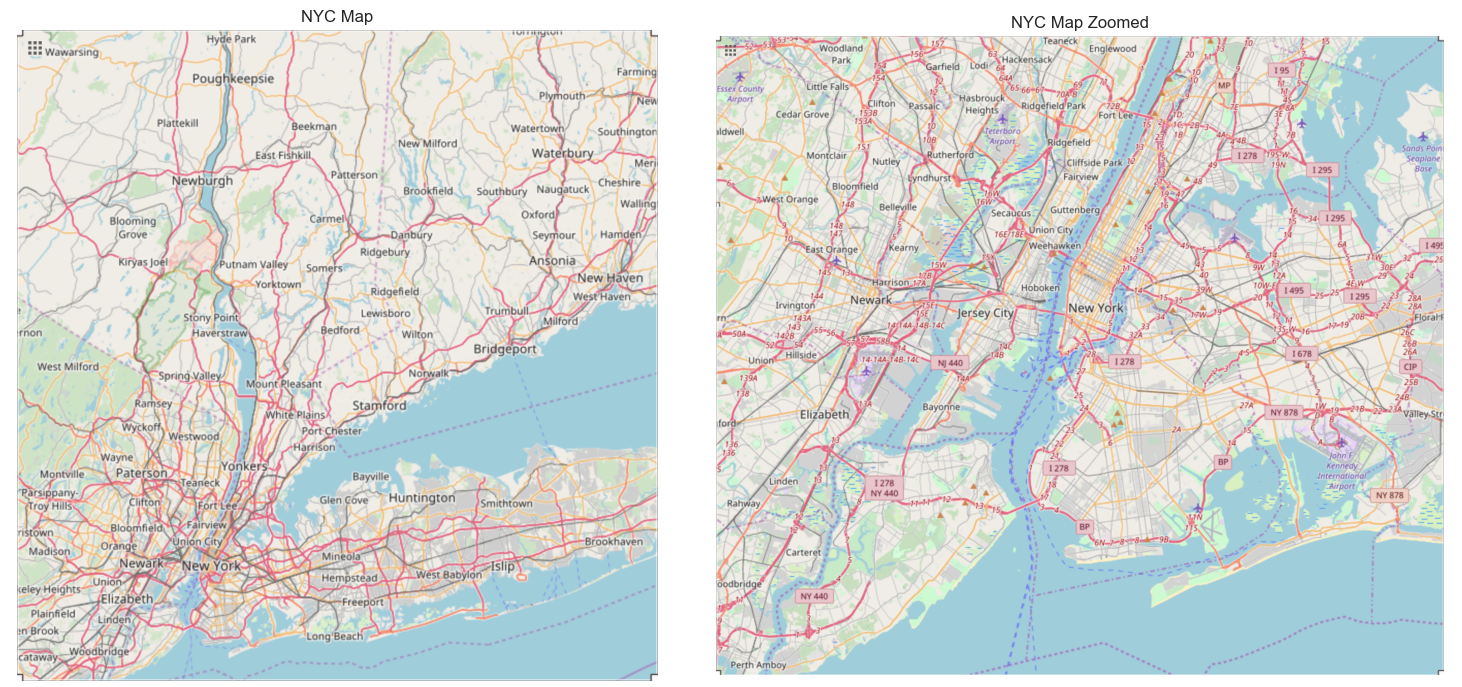
\includegraphics{./Figs/train9.png}
\end{frame}

\begin{frame}[fragile]{Lokacionet}
\protect\hypertarget{lokacionet-8}{}
\AddToHookNext{env/Highlighting/begin}{\tiny}

\begin{Shaded}
\begin{Highlighting}[]
\CommentTok{\# Filtroni të dhënat sipas kutisë së kufizuar dhe shfaqni numrin e rreshtave të rinj}
\BuiltInTok{print}\NormalTok{(}\StringTok{\textquotesingle{}Numri i rreshtave të vjetra: }\SpecialCharTok{\%d}\StringTok{\textquotesingle{}} \OperatorTok{\%} \BuiltInTok{len}\NormalTok{(df\_train))}
\NormalTok{df\_train }\OperatorTok{=}\NormalTok{ df\_train[select\_within\_boundingbox(df\_train, BB)]}
\BuiltInTok{print}\NormalTok{(}\StringTok{\textquotesingle{}Numri i rreshtave të rinj: }\SpecialCharTok{\%d}\StringTok{\textquotesingle{}} \OperatorTok{\%} \BuiltInTok{len}\NormalTok{(df\_train))}
\end{Highlighting}
\end{Shaded}
\end{frame}

\begin{frame}{Lokacionet}
\protect\hypertarget{lokacionet-9}{}
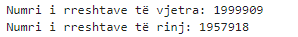
\includegraphics{./Figs/train10.png}
\end{frame}

\begin{frame}[fragile]{Vizualizimi}
\protect\hypertarget{vizualizimi}{}
Vizualizoni të dhënat e trajnimit mbi hartën e NYC duke përdorur
funksionin e mëposhtëm.

\AddToHookNext{env/Highlighting/begin}{\tiny}

\begin{Shaded}
\begin{Highlighting}[]
\CommentTok{\# Funksioni për të vizualizuar të dhënat mbi hartë}
\KeywordTok{def}\NormalTok{ plot\_on\_map(df, BB, nyc\_map, s}\OperatorTok{=}\DecValTok{10}\NormalTok{, alpha}\OperatorTok{=}\FloatTok{0.2}\NormalTok{):}
\NormalTok{    fig, axs }\OperatorTok{=}\NormalTok{ plt.subplots(}\DecValTok{1}\NormalTok{, }\DecValTok{2}\NormalTok{, figsize}\OperatorTok{=}\NormalTok{(}\DecValTok{16}\NormalTok{,}\DecValTok{10}\NormalTok{))}
\NormalTok{    axs[}\DecValTok{0}\NormalTok{].scatter(df.pickup\_longitude, df.pickup\_latitude, zorder}\OperatorTok{=}\DecValTok{1}\NormalTok{, alpha}\OperatorTok{=}\NormalTok{alpha, c}\OperatorTok{=}\StringTok{\textquotesingle{}r\textquotesingle{}}\NormalTok{, s}\OperatorTok{=}\NormalTok{s)}
\NormalTok{    axs[}\DecValTok{0}\NormalTok{].set\_xlim((BB[}\DecValTok{0}\NormalTok{], BB[}\DecValTok{1}\NormalTok{]))}
\NormalTok{    axs[}\DecValTok{0}\NormalTok{].set\_ylim((BB[}\DecValTok{2}\NormalTok{], BB[}\DecValTok{3}\NormalTok{]))}
\NormalTok{    axs[}\DecValTok{0}\NormalTok{].set\_title(}\StringTok{\textquotesingle{}Lokacionet e Marrjes të Taksisë\textquotesingle{}}\NormalTok{)}
\NormalTok{    axs[}\DecValTok{0}\NormalTok{].imshow(nyc\_map, zorder}\OperatorTok{=}\DecValTok{0}\NormalTok{, extent}\OperatorTok{=}\NormalTok{BB)}

\NormalTok{    axs[}\DecValTok{1}\NormalTok{].scatter(df.dropoff\_longitude, df.dropoff\_latitude, zorder}\OperatorTok{=}\DecValTok{1}\NormalTok{, alpha}\OperatorTok{=}\NormalTok{alpha, c}\OperatorTok{=}\StringTok{\textquotesingle{}r\textquotesingle{}}\NormalTok{, s}\OperatorTok{=}\NormalTok{s)}
\NormalTok{    axs[}\DecValTok{1}\NormalTok{].set\_xlim((BB[}\DecValTok{0}\NormalTok{], BB[}\DecValTok{1}\NormalTok{]))}
\NormalTok{    axs[}\DecValTok{1}\NormalTok{].set\_ylim((BB[}\DecValTok{2}\NormalTok{], BB[}\DecValTok{3}\NormalTok{]))}
\NormalTok{    axs[}\DecValTok{1}\NormalTok{].set\_title(}\StringTok{\textquotesingle{}Lokacionet e Zbritjes nga Taksia\textquotesingle{}}\NormalTok{)}
\NormalTok{    axs[}\DecValTok{1}\NormalTok{].imshow(nyc\_map, zorder}\OperatorTok{=}\DecValTok{0}\NormalTok{, extent}\OperatorTok{=}\NormalTok{BB)}
\end{Highlighting}
\end{Shaded}
\end{frame}

\begin{frame}[fragile]{Vizualizimi}
\protect\hypertarget{vizualizimi-1}{}
\AddToHookNext{env/Highlighting/begin}{\tiny}

\begin{Shaded}
\begin{Highlighting}[]
\CommentTok{\# Vizualizoni të dhënat e trajnimit në hartë}
\NormalTok{plot\_on\_map(df\_train, BB, nyc\_map, s}\OperatorTok{=}\DecValTok{1}\NormalTok{, alpha}\OperatorTok{=}\FloatTok{0.3}\NormalTok{)}
\end{Highlighting}
\end{Shaded}
\end{frame}

\begin{frame}{Vizualizimi}
\protect\hypertarget{vizualizimi-2}{}
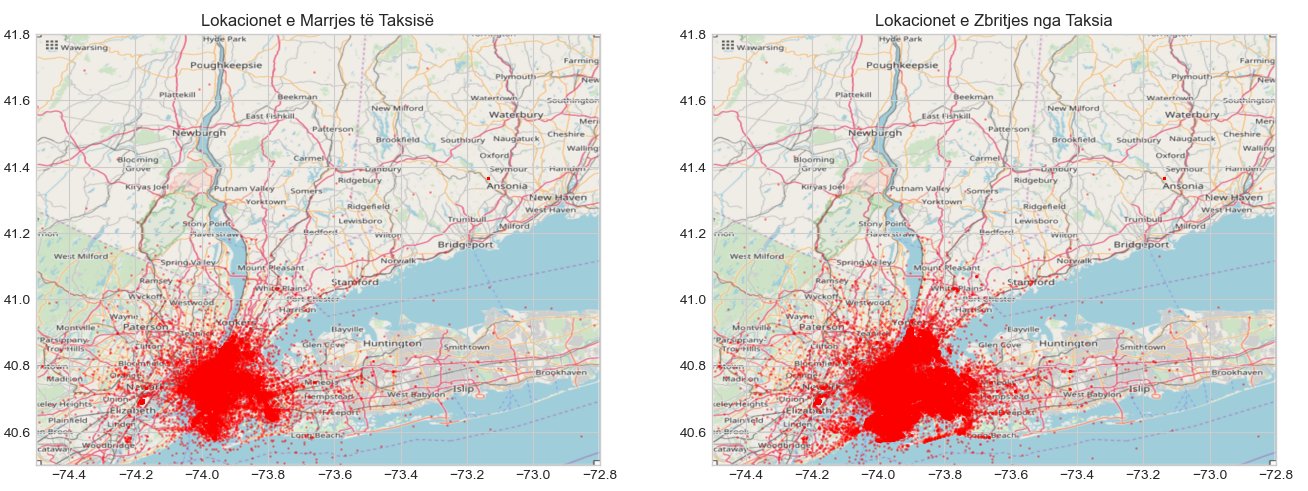
\includegraphics{./Figs/train11.png}
\end{frame}

\begin{frame}[fragile]{Vizualizimi}
\protect\hypertarget{vizualizimi-3}{}
Vizualizimi në hartën e zoom-ur

\AddToHookNext{env/Highlighting/begin}{\tiny}

\begin{Shaded}
\begin{Highlighting}[]
\CommentTok{\# Vizualizoni të dhënat e trajnimit në hartën e zoom}
\NormalTok{plot\_on\_map(df\_test, BB, nyc\_map, alpha}\OperatorTok{=}\FloatTok{1.0}\NormalTok{, s}\OperatorTok{=}\DecValTok{20}\NormalTok{)}
\end{Highlighting}
\end{Shaded}
\end{frame}

\begin{frame}{Vizualizimi}
\protect\hypertarget{vizualizimi-4}{}
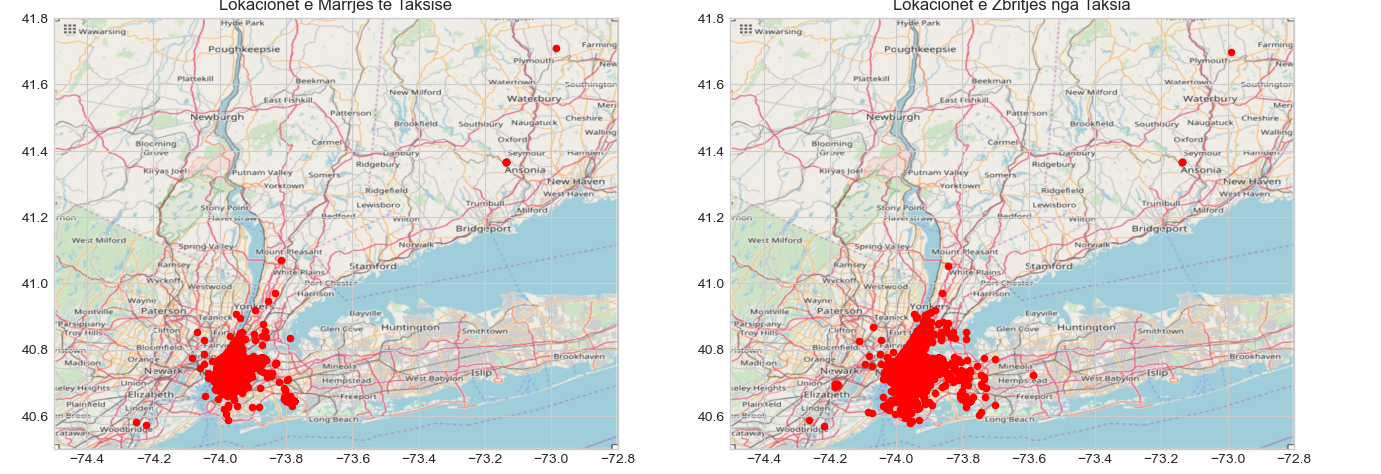
\includegraphics{./Figs/train12.png}
\end{frame}

\begin{frame}{Vizualizimi}
\protect\hypertarget{vizualizimi-5}{}
\begin{itemize}
\item
  Nga grafiku i shpërndarjes së të dhënave të \textbf{train} shohim se
  disa lokacione janë në ujë.
\item
  Ose këto konsiderohen si zhurmë, ose i heqim nga grupi i të dhënave.
\item
  Do t'i heqim në vazhdim
\end{itemize}
\end{frame}

\begin{frame}{Vizualizimi}
\protect\hypertarget{vizualizimi-6}{}
\begin{itemize}
\item
  Një mënyrë tjetër interesante për të vizualizuar të dhënat:
\item
  Duke përdorur përmasa shumë të vogla pikash, rrugët aktuale të Nju
  Jorkut bëhen të dukshme.
\end{itemize}
\end{frame}

\begin{frame}[fragile]{Vizualizimi}
\protect\hypertarget{vizualizimi-7}{}
\AddToHookNext{env/Highlighting/begin}{\tiny}

\begin{Shaded}
\begin{Highlighting}[]
\KeywordTok{def}\NormalTok{ plot\_hires(df, BB, figsize}\OperatorTok{=}\NormalTok{(}\DecValTok{12}\NormalTok{, }\DecValTok{12}\NormalTok{), ax}\OperatorTok{=}\VariableTok{None}\NormalTok{, c}\OperatorTok{=}\NormalTok{(}\StringTok{\textquotesingle{}r\textquotesingle{}}\NormalTok{, }\StringTok{\textquotesingle{}b\textquotesingle{}}\NormalTok{)):}
    \ControlFlowTok{if}\NormalTok{ ax }\OperatorTok{==} \VariableTok{None}\NormalTok{:}
\NormalTok{        fig, ax }\OperatorTok{=}\NormalTok{ plt.subplots(}\DecValTok{1}\NormalTok{, }\DecValTok{1}\NormalTok{, figsize}\OperatorTok{=}\NormalTok{figsize)}

\NormalTok{    idx }\OperatorTok{=}\NormalTok{ select\_within\_boundingbox(df, BB)}
\NormalTok{    ax.scatter(df[idx].pickup\_longitude, df[idx].pickup\_latitude, c}\OperatorTok{=}\NormalTok{c[}\DecValTok{0}\NormalTok{], s}\OperatorTok{=}\FloatTok{0.01}\NormalTok{, alpha}\OperatorTok{=}\FloatTok{0.5}\NormalTok{)}
\NormalTok{    ax.scatter(df[idx].dropoff\_longitude, df[idx].dropoff\_latitude, c}\OperatorTok{=}\NormalTok{c[}\DecValTok{1}\NormalTok{], s}\OperatorTok{=}\FloatTok{0.01}\NormalTok{, alpha}\OperatorTok{=}\FloatTok{0.5}\NormalTok{)}
\end{Highlighting}
\end{Shaded}
\end{frame}

\begin{frame}[fragile]{Vizualizimi}
\protect\hypertarget{vizualizimi-8}{}
\AddToHookNext{env/Highlighting/begin}{\tiny}

\begin{Shaded}
\begin{Highlighting}[]
\NormalTok{plot\_hires(df\_train, (}\OperatorTok{{-}}\FloatTok{74.1}\NormalTok{, }\OperatorTok{{-}}\FloatTok{73.7}\NormalTok{, }\FloatTok{40.6}\NormalTok{, }\FloatTok{40.9}\NormalTok{))}
\NormalTok{plot\_hires(df\_train, (}\OperatorTok{{-}}\DecValTok{74}\NormalTok{, }\OperatorTok{{-}}\FloatTok{73.95}\NormalTok{, }\FloatTok{40.7}\NormalTok{, }\FloatTok{40.8}\NormalTok{))}
\end{Highlighting}
\end{Shaded}
\end{frame}

\begin{frame}{Vizualizimi}
\protect\hypertarget{vizualizimi-9}{}
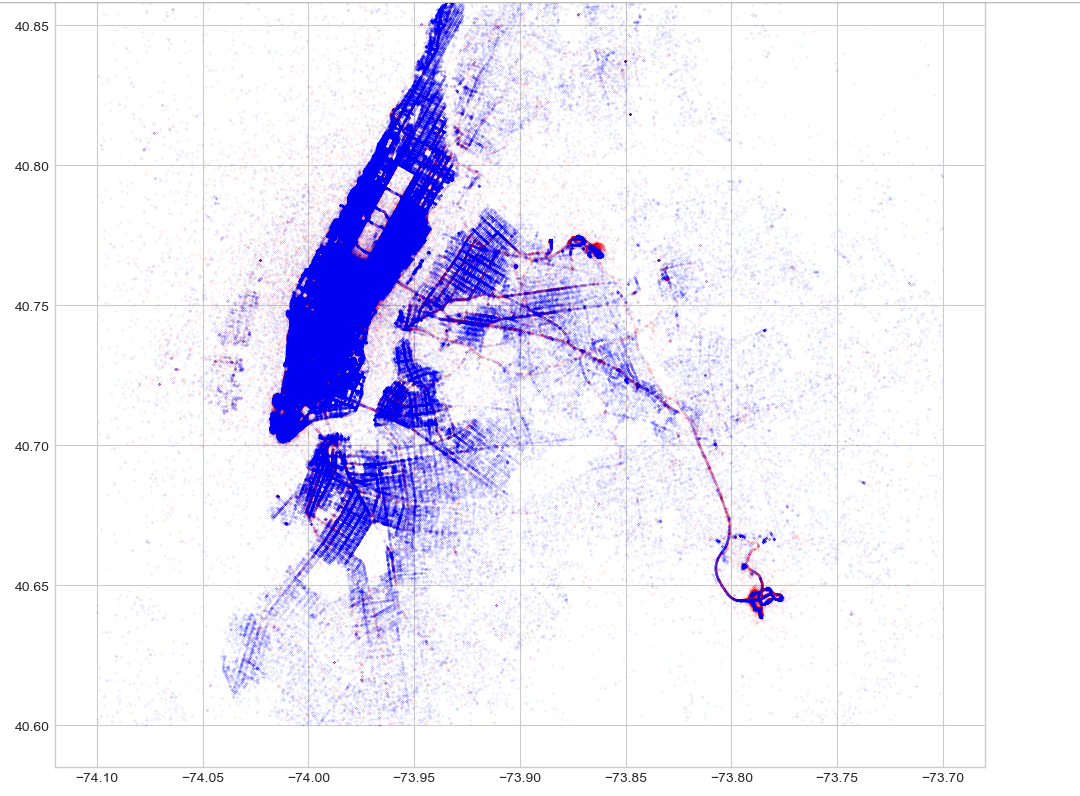
\includegraphics{./Figs/train13.png}
\end{frame}

\begin{frame}{Heqja e pikave të të dhënave në ujë}
\protect\hypertarget{heqja-e-pikave-tuxeb-tuxeb-dhuxebnave-nuxeb-ujuxeb}{}
\begin{itemize}
\item
  Siç mund të shihet nga harta + parcelat e shpërndarjes më sipër, disa
  pika të dhënash ndodhen në ujë.
\item
  Këto janë padyshim pika të dhënash \textbf{noise}.
\item
  Për të hequr këto pika të dhënash, krijojmë një hartë \textbf{boolean}
  tokësore/ujore nga harta e NYC.
\end{itemize}
\end{frame}

\begin{frame}[fragile]{Heqja e pikave të të dhënave në ujë}
\protect\hypertarget{heqja-e-pikave-tuxeb-tuxeb-dhuxebnave-nuxeb-ujuxeb-1}{}
\AddToHookNext{env/Highlighting/begin}{\tiny}

\begin{Shaded}
\begin{Highlighting}[]
\ImportTok{import}\NormalTok{ ssl}
\ImportTok{import}\NormalTok{ urllib.request}
\ImportTok{from}\NormalTok{ PIL }\ImportTok{import}\NormalTok{ Image}
\ImportTok{import}\NormalTok{ numpy }\ImportTok{as}\NormalTok{ np}
\ImportTok{import}\NormalTok{ matplotlib.pyplot }\ImportTok{as}\NormalTok{ plt}

\CommentTok{\# Disable SSL verification temporarily}
\NormalTok{ssl.\_create\_default\_https\_context }\OperatorTok{=}\NormalTok{ ssl.\_create\_unverified\_context}

\CommentTok{\# Function to read image from URL using PIL and urllib}
\KeywordTok{def}\NormalTok{ load\_image(url):}
    \ControlFlowTok{with}\NormalTok{ urllib.request.urlopen(url) }\ImportTok{as}\NormalTok{ url\_data:}
\NormalTok{        img }\OperatorTok{=}\NormalTok{ Image.}\BuiltInTok{open}\NormalTok{(url\_data)}
        \ControlFlowTok{return}\NormalTok{ np.array(img)}

\CommentTok{\# URL of the NYC mask}
\NormalTok{nyc\_mask\_url }\OperatorTok{=} \StringTok{\textquotesingle{}https://aiblog.nl/download/nyc\_mask{-}74.5\_{-}72.8\_40.5\_41.8.png\textquotesingle{}}

\CommentTok{\# Load the mask image and convert to boolean map}
\NormalTok{nyc\_mask\_image }\OperatorTok{=}\NormalTok{ load\_image(nyc\_mask\_url)}
\NormalTok{nyc\_mask }\OperatorTok{=}\NormalTok{ nyc\_mask\_image[:, :, }\DecValTok{0}\NormalTok{] }\OperatorTok{\textgreater{}} \FloatTok{0.9}
\end{Highlighting}
\end{Shaded}
\end{frame}

\begin{frame}[fragile]{Heqja e pikave të të dhënave në ujë (vazhdim)}
\protect\hypertarget{heqja-e-pikave-tuxeb-tuxeb-dhuxebnave-nuxeb-ujuxeb-vazhdim}{}
\AddToHookNext{env/Highlighting/begin}{\tiny}

\begin{Shaded}
\begin{Highlighting}[]
\CommentTok{\# URL e hartës të NYC}
\NormalTok{nyc\_map\_url }\OperatorTok{=} \StringTok{\textquotesingle{}https://aiblog.nl/download/nyc\_{-}74.5\_{-}72.8\_40.5\_41.8.png\textquotesingle{}}
\NormalTok{nyc\_map }\OperatorTok{=}\NormalTok{ load\_image(nyc\_map\_url)}

\CommentTok{\# Ndërtojmë hartën dhe maskën}
\NormalTok{plt.figure(figsize}\OperatorTok{=}\NormalTok{(}\DecValTok{8}\NormalTok{, }\DecValTok{8}\NormalTok{))}
\NormalTok{plt.imshow(nyc\_map, zorder}\OperatorTok{=}\DecValTok{0}\NormalTok{)}
\NormalTok{plt.imshow(nyc\_mask, cmap}\OperatorTok{=}\StringTok{\textquotesingle{}gray\textquotesingle{}}\NormalTok{, zorder}\OperatorTok{=}\DecValTok{1}\NormalTok{, alpha}\OperatorTok{=}\FloatTok{0.3}\NormalTok{)  }\CommentTok{\# Adjust \textasciigrave{}alpha\textasciigrave{} as needed}
\NormalTok{plt.axis(}\StringTok{\textquotesingle{}off\textquotesingle{}}\NormalTok{)}
\NormalTok{plt.title(}\StringTok{\textquotesingle{} Harta e NYC Map me Mask Overlay\textquotesingle{}}\NormalTok{)}
\NormalTok{plt.show()}
\end{Highlighting}
\end{Shaded}
\end{frame}

\begin{frame}{Heqja e pikave të të dhënave në ujë (vazhdim)}
\protect\hypertarget{heqja-e-pikave-tuxeb-tuxeb-dhuxebnave-nuxeb-ujuxeb-vazhdim-1}{}
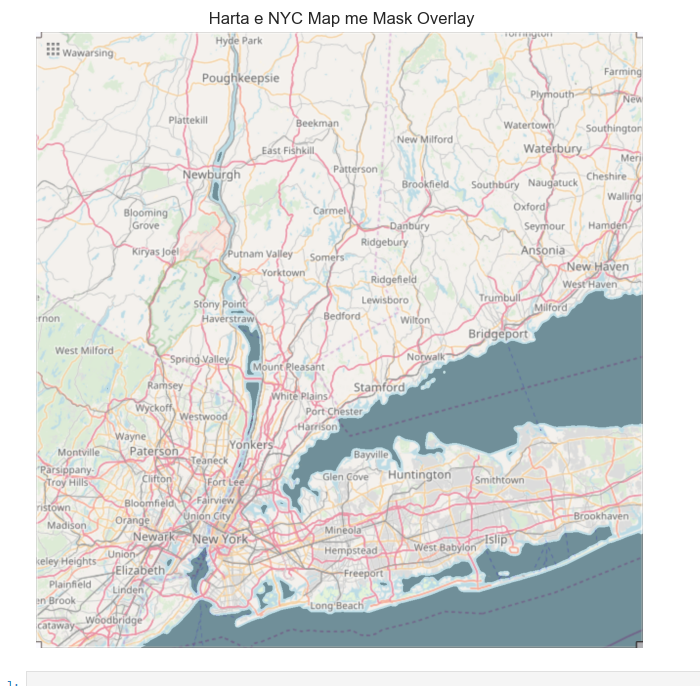
\includegraphics{./Figs/train14.png}
\end{frame}

\begin{frame}{Heqja e pikave të të dhënave në ujë}
\protect\hypertarget{heqja-e-pikave-tuxeb-tuxeb-dhuxebnave-nuxeb-ujuxeb-2}{}
\begin{itemize}
\item
  Më pas, duhet të konvertojmë koordinatat e gjatësisë/gjerësisë
  gjeografike në koordinatat \textbf{piksel xy}.
\item
  Funksioni \textbf{lonlat\_to\_xy} zbaton këtë transformim.
\end{itemize}
\end{frame}

\begin{frame}{Heqja e pikave të të dhënave në ujë}
\protect\hypertarget{heqja-e-pikave-tuxeb-tuxeb-dhuxebnave-nuxeb-ujuxeb-3}{}
\begin{itemize}
\item
  Vini re se koordinata y duhet të kthehet mbrapsht pasi boshti y i
  imazhit drejtohet nga lart poshtë.
\item
  Kur për të gjitha pikat e të dhënave janë llogaritur koordinatat xy
  pixel, një indeks boolean llogaritet duke përdorur maskën NYC.
\end{itemize}
\end{frame}

\begin{frame}[fragile]{Heqja e pikave të të dhënave në ujë}
\protect\hypertarget{heqja-e-pikave-tuxeb-tuxeb-dhuxebnave-nuxeb-ujuxeb-4}{}
\AddToHookNext{env/Highlighting/begin}{\tiny}

\begin{Shaded}
\begin{Highlighting}[]
\CommentTok{\# përktheni koordinatat e gjatësisë/gjerësisë gjeografike në koordinatën xy të imazhit}
\KeywordTok{def}\NormalTok{ lonlat\_to\_xy(longitude, latitude, dx, dy, BB):}
    \ControlFlowTok{return}\NormalTok{ (dx}\OperatorTok{*}\NormalTok{(longitude }\OperatorTok{{-}}\NormalTok{ BB[}\DecValTok{0}\NormalTok{])}\OperatorTok{/}\NormalTok{(BB[}\DecValTok{1}\NormalTok{]}\OperatorTok{{-}}\NormalTok{BB[}\DecValTok{0}\NormalTok{])).astype(}\StringTok{\textquotesingle{}int\textquotesingle{}}\NormalTok{), }\OperatorTok{\textbackslash{}}
\NormalTok{           (dy }\OperatorTok{{-}}\NormalTok{ dy}\OperatorTok{*}\NormalTok{(latitude }\OperatorTok{{-}}\NormalTok{ BB[}\DecValTok{2}\NormalTok{])}\OperatorTok{/}\NormalTok{(BB[}\DecValTok{3}\NormalTok{]}\OperatorTok{{-}}\NormalTok{BB[}\DecValTok{2}\NormalTok{])).astype(}\StringTok{\textquotesingle{}int\textquotesingle{}}\NormalTok{)}
\end{Highlighting}
\end{Shaded}
\end{frame}

\begin{frame}[fragile]{Heqja e pikave të të dhënave në ujë}
\protect\hypertarget{heqja-e-pikave-tuxeb-tuxeb-dhuxebnave-nuxeb-ujuxeb-5}{}
\AddToHookNext{env/Highlighting/begin}{\tiny}

\begin{Shaded}
\begin{Highlighting}[]
\NormalTok{pickup\_x, pickup\_y }\OperatorTok{=}\NormalTok{ lonlat\_to\_xy(df\_train.pickup\_longitude, df\_train.pickup\_latitude, }
\NormalTok{                                  nyc\_mask.shape[}\DecValTok{1}\NormalTok{], nyc\_mask.shape[}\DecValTok{0}\NormalTok{], BB)}
\NormalTok{dropoff\_x, dropoff\_y }\OperatorTok{=}\NormalTok{ lonlat\_to\_xy(df\_train.dropoff\_longitude, df\_train.dropoff\_latitude, }
\NormalTok{                                  nyc\_mask.shape[}\DecValTok{1}\NormalTok{], nyc\_mask.shape[}\DecValTok{0}\NormalTok{], BB)}
\end{Highlighting}
\end{Shaded}
\end{frame}

\begin{frame}[fragile]{Heqja e pikave të të dhënave në ujë}
\protect\hypertarget{heqja-e-pikave-tuxeb-tuxeb-dhuxebnave-nuxeb-ujuxeb-6}{}
\AddToHookNext{env/Highlighting/begin}{\tiny}

\begin{Shaded}
\begin{Highlighting}[]
\NormalTok{idx }\OperatorTok{=}\NormalTok{ (nyc\_mask[pickup\_y, pickup\_x] }\OperatorTok{\&}\NormalTok{ nyc\_mask[dropoff\_y, dropoff\_x])}
\BuiltInTok{print}\NormalTok{(}\StringTok{"Numri i udhëtimeve në ujë: }\SpecialCharTok{\{\}}\StringTok{"}\NormalTok{.}\BuiltInTok{format}\NormalTok{(np.}\BuiltInTok{sum}\NormalTok{(}\OperatorTok{\textasciitilde{}}\NormalTok{idx)))}
\end{Highlighting}
\end{Shaded}
\end{frame}

\begin{frame}{Heqja e pikave të të dhënave në ujë}
\protect\hypertarget{heqja-e-pikave-tuxeb-tuxeb-dhuxebnave-nuxeb-ujuxeb-7}{}
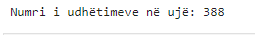
\includegraphics{./Figs/train15.png}
\end{frame}

\begin{frame}{Heqja e pikave të të dhënave në ujë}
\protect\hypertarget{heqja-e-pikave-tuxeb-tuxeb-dhuxebnave-nuxeb-ujuxeb-8}{}
\begin{itemize}
\tightlist
\item
  Krijojmë një funksion që heq pikat e të dhënave nga uji
\end{itemize}
\end{frame}

\begin{frame}[fragile]{Heqja e pikave të të dhënave në ujë}
\protect\hypertarget{heqja-e-pikave-tuxeb-tuxeb-dhuxebnave-nuxeb-ujuxeb-9}{}
\AddToHookNext{env/Highlighting/begin}{\tiny}

\begin{Shaded}
\begin{Highlighting}[]
\ImportTok{import}\NormalTok{ ssl}
\ImportTok{import}\NormalTok{ urllib.request}
\ImportTok{from}\NormalTok{ PIL }\ImportTok{import}\NormalTok{ Image}
\ImportTok{import}\NormalTok{ numpy }\ImportTok{as}\NormalTok{ np}

\CommentTok{\# Çaktivizo përkohësisht verifikimin SSL}
\NormalTok{ssl.\_create\_default\_https\_context }\OperatorTok{=}\NormalTok{ ssl.\_create\_unverified\_context}

\CommentTok{\# Funksioni për të lexuar një imazh nga URL{-}ja duke përdorur PIL dhe urllib}
\KeywordTok{def}\NormalTok{ load\_image(url):}
    \ControlFlowTok{with}\NormalTok{ urllib.request.urlopen(url) }\ImportTok{as}\NormalTok{ url\_data:}
\NormalTok{        img }\OperatorTok{=}\NormalTok{ Image.}\BuiltInTok{open}\NormalTok{(url\_data)}
        \ControlFlowTok{return}\NormalTok{ np.array(img)}

\CommentTok{\# Funksioni i modifikuar remove\_datapoints\_from\_water}
\KeywordTok{def}\NormalTok{ remove\_datapoints\_from\_water(df):}
    \KeywordTok{def}\NormalTok{ lonlat\_to\_xy(longitude, latitude, dx, dy, BB):}
\NormalTok{        x }\OperatorTok{=}\NormalTok{ (dx }\OperatorTok{*}\NormalTok{ (longitude }\OperatorTok{{-}}\NormalTok{ BB[}\DecValTok{0}\NormalTok{]) }\OperatorTok{/}\NormalTok{ (BB[}\DecValTok{1}\NormalTok{] }\OperatorTok{{-}}\NormalTok{ BB[}\DecValTok{0}\NormalTok{])).astype(}\BuiltInTok{int}\NormalTok{)}
\NormalTok{        y }\OperatorTok{=}\NormalTok{ (dy }\OperatorTok{{-}}\NormalTok{ dy }\OperatorTok{*}\NormalTok{ (latitude }\OperatorTok{{-}}\NormalTok{ BB[}\DecValTok{2}\NormalTok{]) }\OperatorTok{/}\NormalTok{ (BB[}\DecValTok{3}\NormalTok{] }\OperatorTok{{-}}\NormalTok{ BB[}\DecValTok{2}\NormalTok{])).astype(}\BuiltInTok{int}\NormalTok{)}
        \CommentTok{\# Sigurohu që koordinatat janë brenda kufijve të imazhit}
\NormalTok{        x }\OperatorTok{=}\NormalTok{ np.clip(x, }\DecValTok{0}\NormalTok{, dx }\OperatorTok{{-}} \DecValTok{1}\NormalTok{)}
\NormalTok{        y }\OperatorTok{=}\NormalTok{ np.clip(y, }\DecValTok{0}\NormalTok{, dy }\OperatorTok{{-}} \DecValTok{1}\NormalTok{)}
        \ControlFlowTok{return}\NormalTok{ x, y}
\end{Highlighting}
\end{Shaded}
\end{frame}

\begin{frame}[fragile]{Heqja e pikave të të dhënave në ujë}
\protect\hypertarget{heqja-e-pikave-tuxeb-tuxeb-dhuxebnave-nuxeb-ujuxeb-10}{}
\AddToHookNext{env/Highlighting/begin}{\tiny}

\begin{Shaded}
\begin{Highlighting}[]
    \CommentTok{\# Defino kutinë e kufizuar (bounding box)}
\NormalTok{    BB }\OperatorTok{=}\NormalTok{ (}\OperatorTok{{-}}\FloatTok{74.5}\NormalTok{, }\OperatorTok{{-}}\FloatTok{72.8}\NormalTok{, }\FloatTok{40.5}\NormalTok{, }\FloatTok{41.8}\NormalTok{)}

    \CommentTok{\# URL{-}ja e maskës së NYC}
\NormalTok{    nyc\_mask\_url }\OperatorTok{=} \StringTok{\textquotesingle{}https://aiblog.nl/download/nyc\_mask{-}74.5\_{-}72.8\_40.5\_41.8.png\textquotesingle{}}

    \CommentTok{\# Ngarko imazhin e maskës dhe ktheje në hartë booleane}
\NormalTok{    nyc\_mask\_image }\OperatorTok{=}\NormalTok{ load\_image(nyc\_mask\_url)}
\NormalTok{    nyc\_mask }\OperatorTok{=}\NormalTok{ nyc\_mask\_image[:, :, }\DecValTok{0}\NormalTok{] }\OperatorTok{\textgreater{}} \FloatTok{0.9}

    \CommentTok{\# Llogarit koordinatat xy të maskës për secilin koordinatë lon/lat}
\NormalTok{    pickup\_x, pickup\_y }\OperatorTok{=}\NormalTok{ lonlat\_to\_xy(df.pickup\_longitude, df.pickup\_latitude, }
\NormalTok{                                      nyc\_mask.shape[}\DecValTok{1}\NormalTok{], nyc\_mask.shape[}\DecValTok{0}\NormalTok{], BB)}
\NormalTok{    dropoff\_x, dropoff\_y }\OperatorTok{=}\NormalTok{ lonlat\_to\_xy(df.dropoff\_longitude, df.dropoff\_latitude, }
\NormalTok{                                      nyc\_mask.shape[}\DecValTok{1}\NormalTok{], nyc\_mask.shape[}\DecValTok{0}\NormalTok{], BB)}
    \CommentTok{\# Llogarit indekset booleane}
\NormalTok{    idx }\OperatorTok{=}\NormalTok{ nyc\_mask[pickup\_y, pickup\_x] }\OperatorTok{\&}\NormalTok{ nyc\_mask[dropoff\_y, dropoff\_x]}

    \CommentTok{\# Kthe vetëm pikat e të dhënave në tokë}
    \ControlFlowTok{return}\NormalTok{ df[idx]}
\end{Highlighting}
\end{Shaded}
\end{frame}

\begin{frame}[fragile]{Heqja e pikave të të dhënave në ujë}
\protect\hypertarget{heqja-e-pikave-tuxeb-tuxeb-dhuxebnave-nuxeb-ujuxeb-11}{}
\AddToHookNext{env/Highlighting/begin}{\tiny}

\begin{Shaded}
\begin{Highlighting}[]
\BuiltInTok{print}\NormalTok{(}\StringTok{\textquotesingle{}Dimensionet e vjetra: }\SpecialCharTok{\%d}\StringTok{\textquotesingle{}} \OperatorTok{\%} \BuiltInTok{len}\NormalTok{(df\_train))}
\NormalTok{df\_train }\OperatorTok{=}\NormalTok{ remove\_datapoints\_from\_water(df\_train)}
\BuiltInTok{print}\NormalTok{(}\StringTok{\textquotesingle{}Dimensionet e reja: }\SpecialCharTok{\%d}\StringTok{\textquotesingle{}} \OperatorTok{\%} \BuiltInTok{len}\NormalTok{(df\_train))}
\end{Highlighting}
\end{Shaded}
\end{frame}

\begin{frame}{Heqja e pikave të të dhënave në ujë}
\protect\hypertarget{heqja-e-pikave-tuxeb-tuxeb-dhuxebnave-nuxeb-ujuxeb-12}{}
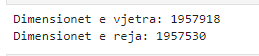
\includegraphics{./Figs/train16.png}
\end{frame}

\begin{frame}[fragile]{Kontrollojmë}
\protect\hypertarget{kontrollojmuxeb}{}
\AddToHookNext{env/Highlighting/begin}{\tiny}

\begin{Shaded}
\begin{Highlighting}[]
\NormalTok{plot\_on\_map(df\_train, BB, nyc\_map)}
\end{Highlighting}
\end{Shaded}
\end{frame}

\begin{frame}{Kontrollojmë}
\protect\hypertarget{kontrollojmuxeb-1}{}
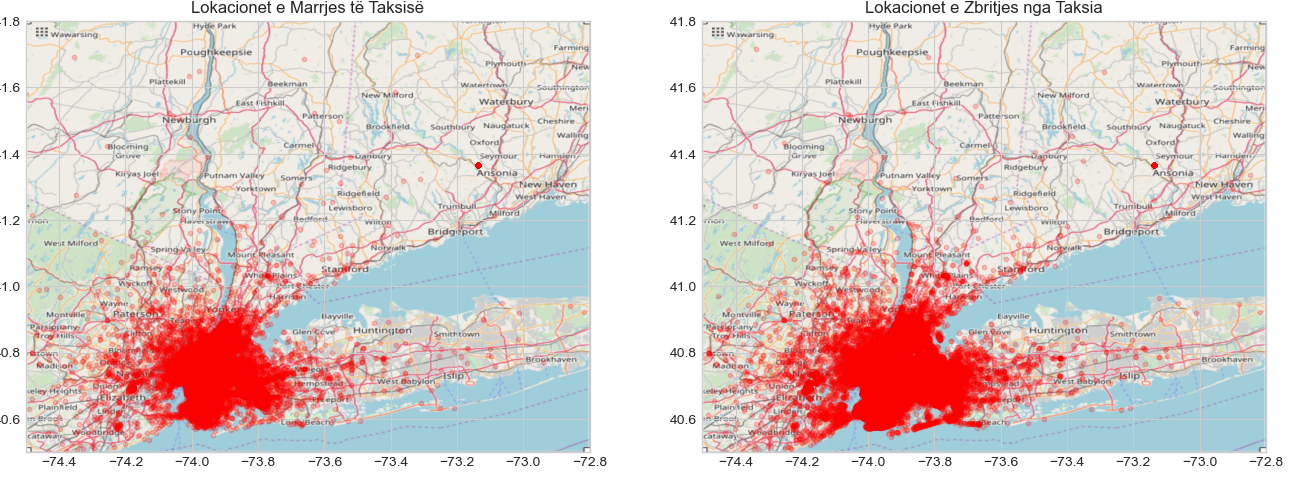
\includegraphics{./Figs/train17.png}
\end{frame}

\begin{frame}{Dendësia e pikave të të dhënave për milje katror}
\protect\hypertarget{denduxebsia-e-pikave-tuxeb-tuxeb-dhuxebnave-puxebr-milje-katror}{}
\begin{itemize}
\item
  Një përmbledhje e lokacioneve të marrjes dhe zbritjes jep një
  përshtypje të shpejtë të densitetit.
\item
  Sidoqoftë, është më e saktë të numërohet numri i pikave të të dhënave
  për zonë për të vizualizuar densitetin.
\end{itemize}
\end{frame}

\begin{frame}{Dendësia e pikave të të dhënave për milje katror}
\protect\hypertarget{denduxebsia-e-pikave-tuxeb-tuxeb-dhuxebnave-puxebr-milje-katror-1}{}
\begin{itemize}
\item
  Kodi më poshtë numëron pikat e të dhënave të marrjes dhe lëshimit për
  milje katrore.
\item
  Kjo jep një pamje më të mirë në `pikat e nxehta'.
\end{itemize}
\end{frame}

\begin{frame}[fragile]{Dendësia e pikave të të dhënave për milje katror}
\protect\hypertarget{denduxebsia-e-pikave-tuxeb-tuxeb-dhuxebnave-puxebr-milje-katror-2}{}
\AddToHookNext{env/Highlighting/begin}{\tiny}

\begin{Shaded}
\begin{Highlighting}[]
\ImportTok{import}\NormalTok{ numpy }\ImportTok{as}\NormalTok{ np}
\ImportTok{import}\NormalTok{ matplotlib.pyplot }\ImportTok{as}\NormalTok{ plt}

\CommentTok{\# Funksioni për të llogaritur distancën në milje midis vendndodhjeve në koordinatat gjerësi, gjatësi}
\CommentTok{\# ktheni distancën në milje}

\KeywordTok{def}\NormalTok{ distance(lat1, lon1, lat2, lon2):}
\NormalTok{    p }\OperatorTok{=} \FloatTok{0.017453292519943295}  \CommentTok{\# Pi/180}
\NormalTok{    a }\OperatorTok{=} \FloatTok{0.5} \OperatorTok{{-}}\NormalTok{ np.cos((lat2 }\OperatorTok{{-}}\NormalTok{ lat1) }\OperatorTok{*}\NormalTok{ p) }\OperatorTok{/} \DecValTok{2} \OperatorTok{+}\NormalTok{ np.cos(lat1 }\OperatorTok{*}\NormalTok{ p) }\OperatorTok{*} 
\NormalTok{    np.cos(lat2 }\OperatorTok{*}\NormalTok{ p) }\OperatorTok{*}\NormalTok{ (}\DecValTok{1} \OperatorTok{{-}}\NormalTok{ np.cos((lon2 }\OperatorTok{{-}}\NormalTok{ lon1) }\OperatorTok{*}\NormalTok{ p)) }\OperatorTok{/} \DecValTok{2}
    \ControlFlowTok{return} \FloatTok{0.6213712} \OperatorTok{*} \DecValTok{12742} \OperatorTok{*}\NormalTok{ np.arcsin(np.sqrt(a))  }\CommentTok{\# 2*R*asin...}

\CommentTok{\# Fillimisht llogaritim dy vektorë me dendësinë e pikave të të dhënave për milje katrore}
\NormalTok{n\_lon, n\_lat }\OperatorTok{=} \DecValTok{200}\NormalTok{, }\DecValTok{200}  \CommentTok{\# numri i koshave të rrjetit për dimensionin gjerësi, gjatësi}
\NormalTok{density\_pickup, density\_dropoff }\OperatorTok{=}\NormalTok{ np.zeros((n\_lat, n\_lon)), np.zeros((n\_lat, n\_lon))  }\CommentTok{\# përgatisni grupet}
\end{Highlighting}
\end{Shaded}
\end{frame}

\begin{frame}[fragile]{Dendësia e pikave të të dhënave për milje katror
(vazhdim)}
\protect\hypertarget{denduxebsia-e-pikave-tuxeb-tuxeb-dhuxebnave-puxebr-milje-katror-vazhdim}{}
\AddToHookNext{env/Highlighting/begin}{\tiny}

\begin{Shaded}
\begin{Highlighting}[]
\CommentTok{\# Për të llogaritur numrin e pikave të të dhënave në një zonë rrjeti, përdoret funksioni numpy.digitize().}
\CommentTok{\# Ky funksion ka nevojë për një vektor me array (vendndodhje) për numërimin e pikave të të dhënave për kosh.}
\NormalTok{bins\_lon }\OperatorTok{=}\NormalTok{ np.zeros(n\_lon }\OperatorTok{+} \DecValTok{1}\NormalTok{)  }\CommentTok{\# koshi}
\NormalTok{bins\_lat }\OperatorTok{=}\NormalTok{ np.zeros(n\_lat }\OperatorTok{+} \DecValTok{1}\NormalTok{)  }\CommentTok{\# koshi}
\NormalTok{delta\_lon }\OperatorTok{=}\NormalTok{ (BB[}\DecValTok{1}\NormalTok{] }\OperatorTok{{-}}\NormalTok{ BB[}\DecValTok{0}\NormalTok{]) }\OperatorTok{/}\NormalTok{ n\_lon  }\CommentTok{\# gjerësia e koshit të gjatë}
\NormalTok{delta\_lat }\OperatorTok{=}\NormalTok{ (BB[}\DecValTok{3}\NormalTok{] }\OperatorTok{{-}}\NormalTok{ BB[}\DecValTok{2}\NormalTok{]) }\OperatorTok{/}\NormalTok{ n\_lat  }\CommentTok{\# lartësia e koshit të gjerësi}
\NormalTok{bin\_width\_miles }\OperatorTok{=}\NormalTok{ distance(BB[}\DecValTok{2}\NormalTok{], BB[}\DecValTok{1}\NormalTok{], BB[}\DecValTok{2}\NormalTok{], BB[}\DecValTok{0}\NormalTok{]) }\OperatorTok{/}\NormalTok{ n\_lon  }\CommentTok{\# gjerësia e koshit në milje}
\NormalTok{bin\_height\_miles }\OperatorTok{=}\NormalTok{ distance(BB[}\DecValTok{3}\NormalTok{], BB[}\DecValTok{0}\NormalTok{], BB[}\DecValTok{2}\NormalTok{], BB[}\DecValTok{0}\NormalTok{]) }\OperatorTok{/}\NormalTok{ n\_lat  }\CommentTok{\# lartësia e koshit në milje}
\ControlFlowTok{for}\NormalTok{ i }\KeywordTok{in} \BuiltInTok{range}\NormalTok{(n\_lon }\OperatorTok{+} \DecValTok{1}\NormalTok{):}
\NormalTok{    bins\_lon[i] }\OperatorTok{=}\NormalTok{ BB[}\DecValTok{0}\NormalTok{] }\OperatorTok{+}\NormalTok{ i }\OperatorTok{*}\NormalTok{ delta\_lon}
\ControlFlowTok{for}\NormalTok{ j }\KeywordTok{in} \BuiltInTok{range}\NormalTok{(n\_lat }\OperatorTok{+} \DecValTok{1}\NormalTok{):}
\NormalTok{    bins\_lat[j] }\OperatorTok{=}\NormalTok{ BB[}\DecValTok{2}\NormalTok{] }\OperatorTok{+}\NormalTok{ j }\OperatorTok{*}\NormalTok{ delta\_lat}
\end{Highlighting}
\end{Shaded}
\end{frame}

\begin{frame}[fragile]{Dendësia e pikave të të dhënave për milje katror
(vazhdim)}
\protect\hypertarget{denduxebsia-e-pikave-tuxeb-tuxeb-dhuxebnave-puxebr-milje-katror-vazhdim-1}{}
\AddToHookNext{env/Highlighting/begin}{\tiny}

\begin{Shaded}
\begin{Highlighting}[]
\CommentTok{\# Ndërtojmë për dimensionin gjatësi, gjerësi}
\NormalTok{inds\_pickup\_lon }\OperatorTok{=}\NormalTok{ np.digitize(df\_train.pickup\_longitude, bins\_lon)}
\NormalTok{inds\_pickup\_lat }\OperatorTok{=}\NormalTok{ np.digitize(df\_train.pickup\_latitude, bins\_lat)}
\NormalTok{inds\_dropoff\_lon }\OperatorTok{=}\NormalTok{ np.digitize(df\_train.dropoff\_longitude, bins\_lon)}
\NormalTok{inds\_dropoff\_lat }\OperatorTok{=}\NormalTok{ np.digitize(df\_train.dropoff\_latitude, bins\_lat)}

\CommentTok{\# Numëroni për array rrjeti}
\CommentTok{\# shënim: mqs density\_pickup do të shfaqet si imazh, indeksi i parë është drejtimi y,}
\CommentTok{\#          indeksi i dytë është drejtimi x. Gjithashtu, drejtimi y duhet të përmbyset për}
\CommentTok{\#          shfaqur si duhet (prandaj termi (n\_lat{-}j))}
\NormalTok{dxdy }\OperatorTok{=}\NormalTok{ bin\_width\_miles }\OperatorTok{*}\NormalTok{ bin\_height\_miles}
\ControlFlowTok{for}\NormalTok{ i }\KeywordTok{in} \BuiltInTok{range}\NormalTok{(n\_lon):}
    \ControlFlowTok{for}\NormalTok{ j }\KeywordTok{in} \BuiltInTok{range}\NormalTok{(n\_lat):}
\NormalTok{        density\_pickup[j, i] }\OperatorTok{=}\NormalTok{ np.}\BuiltInTok{sum}\NormalTok{((inds\_pickup\_lon }\OperatorTok{==}\NormalTok{ i }\OperatorTok{+} \DecValTok{1}\NormalTok{) }\OperatorTok{\&}\NormalTok{ (inds\_pickup\_lat }\OperatorTok{==}\NormalTok{ (n\_lat }\OperatorTok{{-}}\NormalTok{ j))) }\OperatorTok{/}\NormalTok{ dxdy}
\NormalTok{        density\_dropoff[j, i] }\OperatorTok{=}\NormalTok{ np.}\BuiltInTok{sum}\NormalTok{((inds\_dropoff\_lon }\OperatorTok{==}\NormalTok{ i }\OperatorTok{+} \DecValTok{1}\NormalTok{) }\OperatorTok{\&}\NormalTok{ (inds\_dropoff\_lat }\OperatorTok{==}\NormalTok{ (n\_lat }\OperatorTok{{-}}\NormalTok{ j))) }\OperatorTok{/}\NormalTok{ dxdy}

\CommentTok{\# Vizato grupet e dendësisë}
\NormalTok{fig, axs }\OperatorTok{=}\NormalTok{ plt.subplots(}\DecValTok{2}\NormalTok{, }\DecValTok{1}\NormalTok{, figsize}\OperatorTok{=}\NormalTok{(}\DecValTok{18}\NormalTok{, }\DecValTok{24}\NormalTok{))}
\NormalTok{axs[}\DecValTok{0}\NormalTok{].imshow(nyc\_map, zorder}\OperatorTok{=}\DecValTok{0}\NormalTok{, extent}\OperatorTok{=}\NormalTok{BB)}
\NormalTok{im }\OperatorTok{=}\NormalTok{ axs[}\DecValTok{0}\NormalTok{].imshow(np.log1p(density\_pickup), zorder}\OperatorTok{=}\DecValTok{1}\NormalTok{, extent}\OperatorTok{=}\NormalTok{BB, alpha}\OperatorTok{=}\FloatTok{0.6}\NormalTok{, cmap}\OperatorTok{=}\StringTok{\textquotesingle{}plasma\textquotesingle{}}\NormalTok{)}
\NormalTok{axs[}\DecValTok{0}\NormalTok{].set\_title(}\StringTok{\textquotesingle{}Dendësia e marrjes [pika të dhënash për milje katrore]\textquotesingle{}}\NormalTok{)}
\NormalTok{cbar }\OperatorTok{=}\NormalTok{ fig.colorbar(im, ax}\OperatorTok{=}\NormalTok{axs[}\DecValTok{0}\NormalTok{])}
\NormalTok{cbar.set\_label(}\StringTok{\textquotesingle{}log(1 + \#pikave të dhënash për milje katrore)\textquotesingle{}}\NormalTok{, rotation}\OperatorTok{=}\DecValTok{270}\NormalTok{)}
\end{Highlighting}
\end{Shaded}
\end{frame}

\begin{frame}[fragile]{Dendësia e pikave të të dhënave për milje katror
(vazhdim)}
\protect\hypertarget{denduxebsia-e-pikave-tuxeb-tuxeb-dhuxebnave-puxebr-milje-katror-vazhdim-2}{}
\AddToHookNext{env/Highlighting/begin}{\tiny}

\begin{Shaded}
\begin{Highlighting}[]
\NormalTok{axs[}\DecValTok{1}\NormalTok{].imshow(nyc\_map, zorder}\OperatorTok{=}\DecValTok{0}\NormalTok{, extent}\OperatorTok{=}\NormalTok{BB)}
\NormalTok{im }\OperatorTok{=}\NormalTok{ axs[}\DecValTok{1}\NormalTok{].imshow(np.log1p(density\_dropoff), zorder}\OperatorTok{=}\DecValTok{1}\NormalTok{, extent}\OperatorTok{=}\NormalTok{BB, alpha}\OperatorTok{=}\FloatTok{0.6}\NormalTok{, cmap}\OperatorTok{=}\StringTok{\textquotesingle{}plasma\textquotesingle{}}\NormalTok{)}
\NormalTok{axs[}\DecValTok{1}\NormalTok{].set\_title(}\StringTok{\textquotesingle{}Dendësia e zbritjes [pika të dhënash për milje katrore]\textquotesingle{}}\NormalTok{)}
\NormalTok{cbar }\OperatorTok{=}\NormalTok{ fig.colorbar(im, ax}\OperatorTok{=}\NormalTok{axs[}\DecValTok{1}\NormalTok{])}
\NormalTok{cbar.set\_label(}\StringTok{\textquotesingle{}log(1 + \#pikave të dhënash për milje katrore)\textquotesingle{}}\NormalTok{, rotation}\OperatorTok{=}\DecValTok{270}\NormalTok{)}
\end{Highlighting}
\end{Shaded}
\end{frame}

\begin{frame}{Dendësia e pikave të të dhënave për milje katror
(vazhdim)}
\protect\hypertarget{denduxebsia-e-pikave-tuxeb-tuxeb-dhuxebnave-puxebr-milje-katror-vazhdim-3}{}
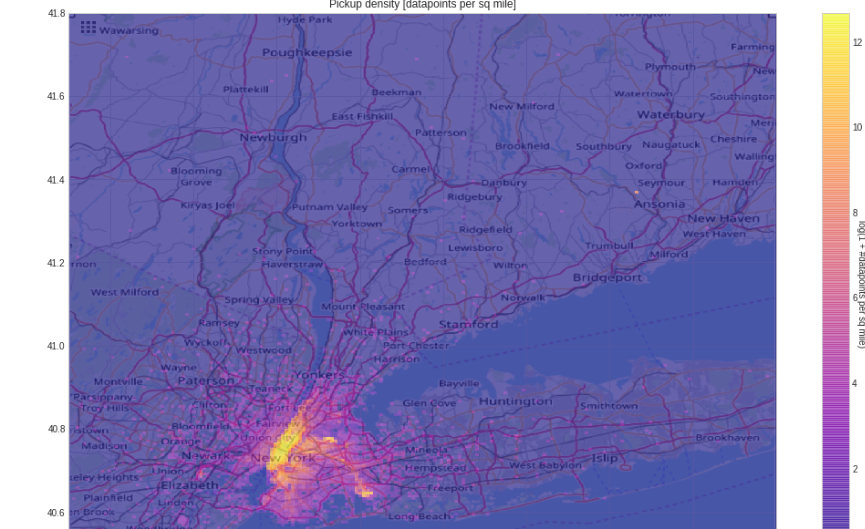
\includegraphics{./Figs/train18.png}
\end{frame}

\begin{frame}{Dendësia e pikave të të dhënave për milje katror
(vazhdim)}
\protect\hypertarget{denduxebsia-e-pikave-tuxeb-tuxeb-dhuxebnave-puxebr-milje-katror-vazhdim-4}{}
\begin{itemize}
\item
  Këto harta tregojnë qartë se pikat e të dhënave përqendrohen rreth
  Manhatenit dhe tre aeroporteve (JFK, EWS, LGR).
\item
  Ekziston gjithashtu një pikë e nxehtë pranë Seymour (këndi i sipërm i
  djathtë).
\item
  Meqenëse nuk jam nga SHBA-ja, a ka dikush një ide se çfarë është kaq e
  veçantë për këtë vendndodhje?
\end{itemize}
\end{frame}

\begin{frame}{Dendësia e trafikut të marrjes}
\protect\hypertarget{denduxebsia-e-trafikut-tuxeb-marrjes}{}
\begin{itemize}
\item
  Grafikët e dendësisë së mësipërme na nxitin të shohim nëse mund ta
  përfytyrojmë densitetin e trafikut për orë (dhe vit).
\item
  Duke numëruar numrin e marrjeve të taksive në një zonë, duhet të kemi
  një përshtypje të densitetit të trafikut.
\item
  Sa më shumë trafik, aq më shumë mund të duhet për të bërë një rrugë.
\end{itemize}
\end{frame}

\begin{frame}[fragile]{Dendësia e trafikut të marrjes}
\protect\hypertarget{denduxebsia-e-trafikut-tuxeb-marrjes-1}{}
\AddToHookNext{env/Highlighting/begin}{\tiny}

\begin{Shaded}
\begin{Highlighting}[]
\CommentTok{\# shtojmë info për kohën}
\NormalTok{df\_train[}\StringTok{\textquotesingle{}year\textquotesingle{}}\NormalTok{] }\OperatorTok{=}\NormalTok{ df\_train.pickup\_datetime.}\BuiltInTok{apply}\NormalTok{(}\KeywordTok{lambda}\NormalTok{ t: t.year)}
\NormalTok{df\_train[}\StringTok{\textquotesingle{}weekday\textquotesingle{}}\NormalTok{] }\OperatorTok{=}\NormalTok{ df\_train.pickup\_datetime.}\BuiltInTok{apply}\NormalTok{(}\KeywordTok{lambda}\NormalTok{ t: t.weekday())}
\NormalTok{df\_train[}\StringTok{\textquotesingle{}hour\textquotesingle{}}\NormalTok{] }\OperatorTok{=}\NormalTok{ df\_train.pickup\_datetime.}\BuiltInTok{apply}\NormalTok{(}\KeywordTok{lambda}\NormalTok{ t: t.hour)}
\end{Highlighting}
\end{Shaded}
\end{frame}

\begin{frame}[fragile]{Dendësia e trafikut të marrjes}
\protect\hypertarget{denduxebsia-e-trafikut-tuxeb-marrjes-2}{}
\AddToHookNext{env/Highlighting/begin}{\tiny}

\begin{Shaded}
\begin{Highlighting}[]
\CommentTok{\# disa konstante të nevojshme për të llogaritur dendësinë e trafikut të marrjes}
\NormalTok{n\_hours }\OperatorTok{=} \DecValTok{24}
\NormalTok{n\_weekdays }\OperatorTok{=} \DecValTok{7}
\NormalTok{n\_years }\OperatorTok{=} \DecValTok{7}
\NormalTok{n\_bins\_lon }\OperatorTok{=} \DecValTok{30}
\NormalTok{n\_bins\_lat }\OperatorTok{=} \DecValTok{30}

\CommentTok{\# fokusimi në trafikun në Manhattan}
\NormalTok{BB\_traffic }\OperatorTok{=}\NormalTok{ (}\OperatorTok{{-}}\FloatTok{74.025}\NormalTok{, }\OperatorTok{{-}}\FloatTok{73.925}\NormalTok{, }\FloatTok{40.7}\NormalTok{, }\FloatTok{40.8}\NormalTok{)}
\end{Highlighting}
\end{Shaded}
\end{frame}

\begin{frame}[fragile]{Dendësia e trafikut të marrjes}
\protect\hypertarget{denduxebsia-e-trafikut-tuxeb-marrjes-3}{}
\AddToHookNext{env/Highlighting/begin}{\tiny}

\begin{Shaded}
\begin{Highlighting}[]
\CommentTok{\# përkufizo funksionin për të llogaritur dendësinë e trafikut të marrjes}
\KeywordTok{def}\NormalTok{ calculate\_trafic\_density(df):}
\NormalTok{    traffic }\OperatorTok{=}\NormalTok{ np.zeros((n\_years, n\_weekdays, n\_hours, n\_bins\_lat, n\_bins\_lon))}
    
    \CommentTok{\# Për të llogaritur numrin e pikave të të dhënave në një zonë rrjeti, përdoret funksioni numpy.digitize().}
    \CommentTok{\# Ky funksion ka nevojë për një vektor me kosha (vendndodhje) për numërimin e pikave të të dhënave}
    \CommentTok{\# për kosh.}
\NormalTok{    bins\_lon }\OperatorTok{=}\NormalTok{ np.zeros(n\_bins\_lon}\OperatorTok{+}\DecValTok{1}\NormalTok{)  }\CommentTok{\# koshi}
\NormalTok{    bins\_lat }\OperatorTok{=}\NormalTok{ np.zeros(n\_bins\_lat}\OperatorTok{+}\DecValTok{1}\NormalTok{)  }\CommentTok{\# koshi}
    
\NormalTok{    delta\_lon }\OperatorTok{=}\NormalTok{ (BB\_traffic[}\DecValTok{1}\NormalTok{] }\OperatorTok{{-}}\NormalTok{ BB\_traffic[}\DecValTok{0}\NormalTok{]) }\OperatorTok{/}\NormalTok{ n\_bins\_lon  }\CommentTok{\# gjerësia e koshit të gjatë}
\NormalTok{    delta\_lat }\OperatorTok{=}\NormalTok{ (BB\_traffic[}\DecValTok{3}\NormalTok{] }\OperatorTok{{-}}\NormalTok{ BB\_traffic[}\DecValTok{2}\NormalTok{]) }\OperatorTok{/}\NormalTok{ n\_bins\_lat  }\CommentTok{\# lartësia e koshit të gjerësi}
    
    \ControlFlowTok{for}\NormalTok{ i }\KeywordTok{in} \BuiltInTok{range}\NormalTok{(n\_bins\_lon}\OperatorTok{+}\DecValTok{1}\NormalTok{):}
\NormalTok{        bins\_lon[i] }\OperatorTok{=}\NormalTok{ BB\_traffic[}\DecValTok{0}\NormalTok{] }\OperatorTok{+}\NormalTok{ i }\OperatorTok{*}\NormalTok{ delta\_lon}
    \ControlFlowTok{for}\NormalTok{ j }\KeywordTok{in} \BuiltInTok{range}\NormalTok{(n\_bins\_lat}\OperatorTok{+}\DecValTok{1}\NormalTok{):}
\NormalTok{        bins\_lat[j] }\OperatorTok{=}\NormalTok{ BB\_traffic[}\DecValTok{2}\NormalTok{] }\OperatorTok{+}\NormalTok{ j }\OperatorTok{*}\NormalTok{ delta\_lat}
\end{Highlighting}
\end{Shaded}
\end{frame}

\begin{frame}[fragile]{Dendësia e trafikut të marrjes (vazhdim)}
\protect\hypertarget{denduxebsia-e-trafikut-tuxeb-marrjes-vazhdim}{}
\AddToHookNext{env/Highlighting/begin}{\tiny}

\begin{Shaded}
\begin{Highlighting}[]
    \CommentTok{\# Numëroni për kosh rrjeti}
    \CommentTok{\# shënim: pasi që density\_pickup do të shfaqet si imazh, indeksi i parë është drejtimi y,}
    \CommentTok{\#          indeksi i dytë është drejtimi x. Gjithashtu, drejtimi y duhet të përmbyset për}
    \CommentTok{\#          shfaqur si duhet (prandaj termi (n\_lat{-}j))}
    \ControlFlowTok{for}\NormalTok{ y }\KeywordTok{in} \BuiltInTok{range}\NormalTok{(n\_years):}
        \ControlFlowTok{for}\NormalTok{ d }\KeywordTok{in} \BuiltInTok{range}\NormalTok{(n\_weekdays):}
            \ControlFlowTok{for}\NormalTok{ h }\KeywordTok{in} \BuiltInTok{range}\NormalTok{(n\_hours):}
\NormalTok{                idx }\OperatorTok{=}\NormalTok{ (df.year }\OperatorTok{==}\NormalTok{ (}\DecValTok{2009} \OperatorTok{+}\NormalTok{ y)) }\OperatorTok{\&}\NormalTok{ (df.weekday }\OperatorTok{==}\NormalTok{ d) }\OperatorTok{\&}\NormalTok{ (df.hour }\OperatorTok{==}\NormalTok{ h)}

                \CommentTok{\# Digjitoni për dimensionin gjatësi, gjerësi}
\NormalTok{                inds\_pickup\_lon }\OperatorTok{=}\NormalTok{ np.digitize(df[idx].pickup\_longitude, bins\_lon)}
\NormalTok{                inds\_pickup\_lat }\OperatorTok{=}\NormalTok{ np.digitize(df[idx].pickup\_latitude, bins\_lat)}

                \ControlFlowTok{for}\NormalTok{ i }\KeywordTok{in} \BuiltInTok{range}\NormalTok{(n\_bins\_lon):}
                    \ControlFlowTok{for}\NormalTok{ j }\KeywordTok{in} \BuiltInTok{range}\NormalTok{(n\_bins\_lat):}
\NormalTok{                        traffic[y, d, h, j, i] }\OperatorTok{=}\NormalTok{ traffic[y, d, h, j, i] }\OperatorTok{+} \OperatorTok{\textbackslash{}}
\NormalTok{                                                 np.}\BuiltInTok{sum}\NormalTok{((inds\_pickup\_lon }\OperatorTok{==}\NormalTok{ i }\OperatorTok{+} \DecValTok{1}\NormalTok{) }\OperatorTok{\&}\NormalTok{ (inds\_pickup\_lat }\OperatorTok{==}\NormalTok{ j }\OperatorTok{+} \DecValTok{1}\NormalTok{))}
    
    \ControlFlowTok{return}\NormalTok{ traffic}
\end{Highlighting}
\end{Shaded}
\end{frame}

\begin{frame}[fragile]{Dendësia e trafikut të marrjes (vazhdim)}
\protect\hypertarget{denduxebsia-e-trafikut-tuxeb-marrjes-vazhdim-1}{}
\AddToHookNext{env/Highlighting/begin}{\tiny}

\begin{Shaded}
\begin{Highlighting}[]
\CommentTok{\# përkufizo funksionin për të vizatuar dendësinë e trafikut të marrjes}
\KeywordTok{def}\NormalTok{ plot\_traffic(traffic, y, d):}
\NormalTok{    days }\OperatorTok{=}\NormalTok{ \{}\StringTok{\textquotesingle{}monday\textquotesingle{}}\NormalTok{: }\DecValTok{0}\NormalTok{, }\StringTok{\textquotesingle{}tuesday\textquotesingle{}}\NormalTok{: }\DecValTok{1}\NormalTok{, }\StringTok{\textquotesingle{}wednesday\textquotesingle{}}\NormalTok{: }\DecValTok{2}\NormalTok{, }\StringTok{\textquotesingle{}thursday\textquotesingle{}}\NormalTok{: }\DecValTok{3}\NormalTok{, }\StringTok{\textquotesingle{}friday\textquotesingle{}}\NormalTok{: }\DecValTok{4}\NormalTok{, }\StringTok{\textquotesingle{}saturday\textquotesingle{}}\NormalTok{: }\DecValTok{5}\NormalTok{, }\StringTok{\textquotesingle{}sunday\textquotesingle{}}\NormalTok{: }\DecValTok{6}\NormalTok{\}}
\NormalTok{    fig, axs }\OperatorTok{=}\NormalTok{ plt.subplots(}\DecValTok{3}\NormalTok{, }\DecValTok{8}\NormalTok{, figsize}\OperatorTok{=}\NormalTok{(}\DecValTok{18}\NormalTok{, }\DecValTok{7}\NormalTok{))}
\NormalTok{    axs }\OperatorTok{=}\NormalTok{ axs.ravel()}
    \ControlFlowTok{for}\NormalTok{ h }\KeywordTok{in} \BuiltInTok{range}\NormalTok{(}\DecValTok{24}\NormalTok{):}
\NormalTok{        axs[h].imshow(traffic[y }\OperatorTok{{-}} \DecValTok{2009}\NormalTok{, days[d], h, ::}\OperatorTok{{-}}\DecValTok{1}\NormalTok{, :], zorder}\OperatorTok{=}\DecValTok{1}\NormalTok{, cmap}\OperatorTok{=}\StringTok{\textquotesingle{}coolwarm\textquotesingle{}}\NormalTok{, clim}\OperatorTok{=}\NormalTok{(}\DecValTok{0}\NormalTok{, traffic.}\BuiltInTok{max}\NormalTok{()))}
\NormalTok{        axs[h].get\_xaxis().set\_visible(}\VariableTok{False}\NormalTok{)}
\NormalTok{        axs[h].get\_yaxis().set\_visible(}\VariableTok{False}\NormalTok{)}
\NormalTok{        axs[h].set\_title(}\StringTok{\textquotesingle{}h=}\SpecialCharTok{\{\}}\StringTok{\textquotesingle{}}\NormalTok{.}\BuiltInTok{format}\NormalTok{(h))}
\NormalTok{    fig.suptitle(}\StringTok{"Dendësia e trafikut të marrjes, viti=}\SpecialCharTok{\{\}}\StringTok{, dita=}\SpecialCharTok{\{\}}\StringTok{ (max\_pickups=}\SpecialCharTok{\{\}}\StringTok{)"}\NormalTok{.}\BuiltInTok{format}\NormalTok{(y, d, traffic.}\BuiltInTok{max}\NormalTok{()))}
\end{Highlighting}
\end{Shaded}
\end{frame}

\begin{frame}{Dendësia e trafikut të marrjes}
\protect\hypertarget{denduxebsia-e-trafikut-tuxeb-marrjes-4}{}
\begin{itemize}
\item
  Tani, le të llogarisim densitetin dhe të përfytyrojmë parcelat.
\item
  cilësia e grafikëve varet nga numri i pikave të të dhënave të
  përdorura.
\end{itemize}
\end{frame}

\begin{frame}{Dendësia e trafikut të marrjes}
\protect\hypertarget{denduxebsia-e-trafikut-tuxeb-marrjes-5}{}
\begin{itemize}
\item
  Përdorim si parazgjedhje 500 mijë pika, të cilat nuk mjaftojnë për
  parcela me densitet të mirë trafiku.
\item
  Rritni numrin e pikëve dhe merrni parcela më të mira.
\end{itemize}
\end{frame}

\begin{frame}[fragile]{Dendësia e trafikut të marrjes}
\protect\hypertarget{denduxebsia-e-trafikut-tuxeb-marrjes-6}{}
\AddToHookNext{env/Highlighting/begin}{\tiny}

\begin{Shaded}
\begin{Highlighting}[]
\NormalTok{traffic }\OperatorTok{=}\NormalTok{ calculate\_trafic\_density(df\_train)}
\NormalTok{plot\_traffic(traffic, }\DecValTok{2009}\NormalTok{, }\StringTok{\textquotesingle{}monday\textquotesingle{}}\NormalTok{)}
\NormalTok{plot\_traffic(traffic, }\DecValTok{2009}\NormalTok{, }\StringTok{\textquotesingle{}friday\textquotesingle{}}\NormalTok{)}
\NormalTok{plot\_traffic(traffic, }\DecValTok{2009}\NormalTok{, }\StringTok{\textquotesingle{}sunday\textquotesingle{}}\NormalTok{)}
\end{Highlighting}
\end{Shaded}
\end{frame}

\begin{frame}{Dendësia e trafikut të marrjes}
\protect\hypertarget{denduxebsia-e-trafikut-tuxeb-marrjes-7}{}
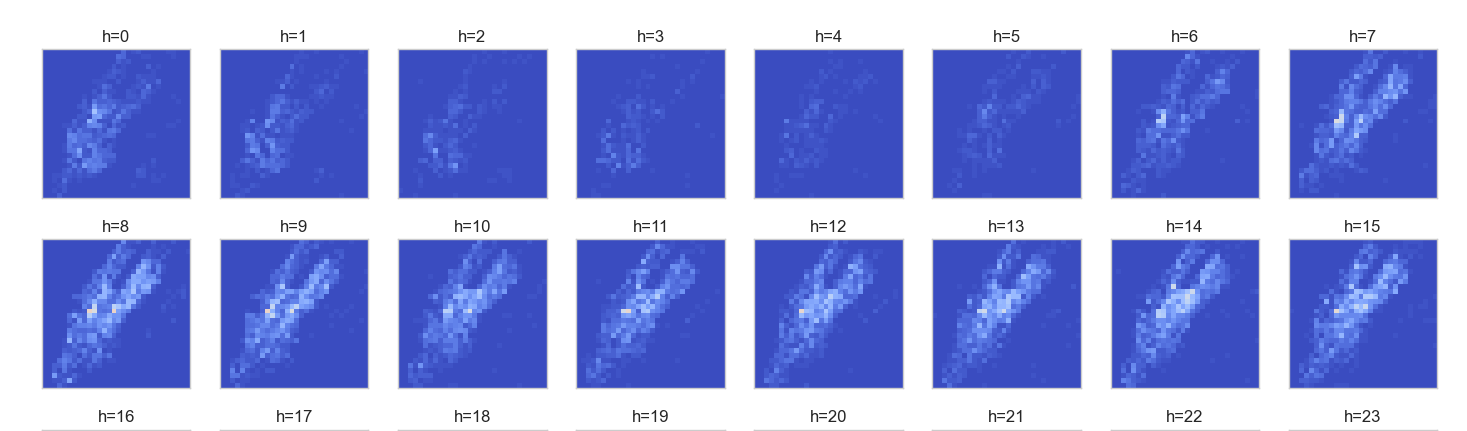
\includegraphics{./Figs/train19.png}
\end{frame}

\begin{frame}{Dendësia e trafikut të marrjes}
\protect\hypertarget{denduxebsia-e-trafikut-tuxeb-marrjes-8}{}
\begin{itemize}
\item
  Tashmë nga këto parcela mund të shohim modelet e ndryshme të
  densitetit të trafikut sipas orës, por edhe sipas vendndodhjes.
\item
  P.sh. të dielën h=0-3 orë (e shtunë mbrëma deri të dielën) ka më shumë
  trafik se në ditët e javës.
\end{itemize}
\end{frame}

\begin{frame}{Dendësia e trafikut të marrjes}
\protect\hypertarget{denduxebsia-e-trafikut-tuxeb-marrjes-9}{}
\begin{itemize}
\item
  Supozojmë se kjo është nga njerëzit që dalin dhe shijojnë fundjavën.
\item
  Le të përfytyrojmë edhe një vit tjetër.
\end{itemize}
\end{frame}

\begin{frame}[fragile]{Dendësia e trafikut të marrjes}
\protect\hypertarget{denduxebsia-e-trafikut-tuxeb-marrjes-10}{}
\AddToHookNext{env/Highlighting/begin}{\tiny}

\begin{Shaded}
\begin{Highlighting}[]
\NormalTok{plot\_traffic(traffic, }\DecValTok{2014}\NormalTok{, }\StringTok{\textquotesingle{}monday\textquotesingle{}}\NormalTok{)}
\NormalTok{plot\_traffic(traffic, }\DecValTok{2014}\NormalTok{, }\StringTok{\textquotesingle{}friday\textquotesingle{}}\NormalTok{)}
\NormalTok{plot\_traffic(traffic, }\DecValTok{2014}\NormalTok{, }\StringTok{\textquotesingle{}sunday\textquotesingle{}}\NormalTok{)}
\end{Highlighting}
\end{Shaded}
\end{frame}

\begin{frame}{Dendësia e trafikut të marrjes}
\protect\hypertarget{denduxebsia-e-trafikut-tuxeb-marrjes-11}{}
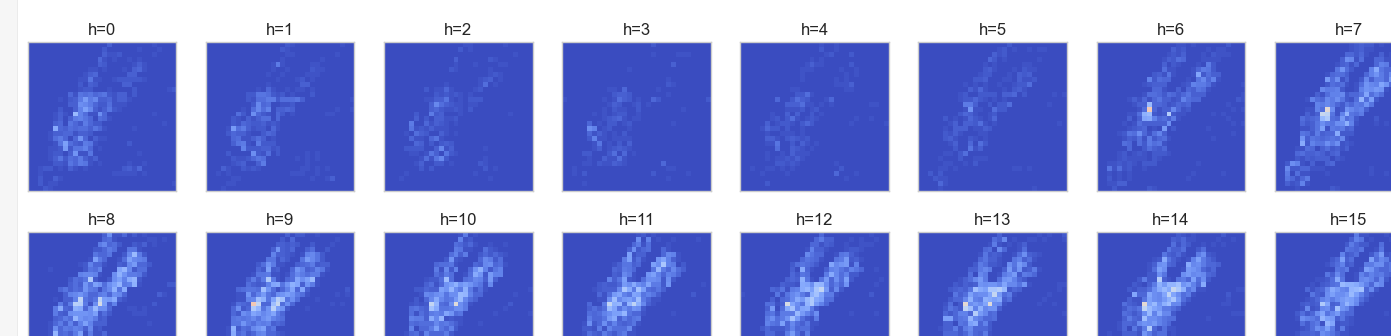
\includegraphics{./Figs/train20.png}
\end{frame}

\begin{frame}{Analiza e Dendësisë dhe Distancës së Trafikut''}
\protect\hypertarget{analiza-e-denduxebsisuxeb-dhe-distancuxebs-suxeb-trafikut}{}
Përpara se të ndërtojmë një model, duam të testojmë disa `intuicione':

\begin{itemize}
\item
  Sa më e gjatë distanca midis vendndodhjes së marrjes dhe zbritjes, aq
  më i lartë është çmimi.
\item
  Disa udhëtime, si p.sh. nga/te një aeroport, kanë tarifa të
  përcaktuara.
\item
  Tarifa gjatë natës është ndryshe nga ajo e ditës.
\end{itemize}
\end{frame}

\begin{frame}{Analiza e Dendësisë dhe Distancës së Trafikut''}
\protect\hypertarget{analiza-e-denduxebsisuxeb-dhe-distancuxebs-suxeb-trafikut-1}{}
\begin{itemize}
\tightlist
\item
  Pra, le të kontrollojmë.
\end{itemize}
\end{frame}

\begin{frame}{Distanca dhe Çmimi}
\protect\hypertarget{distanca-dhe-uxe7mimi}{}
\begin{itemize}
\tightlist
\item
  Sa më e gjatë distanca midis vendndodhjes së marrjes dhe zbritjes, aq
  më i lartë është çmimi.
\end{itemize}
\end{frame}

\begin{frame}[fragile]{Distanca dhe Çmimi}
\protect\hypertarget{distanca-dhe-uxe7mimi-1}{}
Për të vizualizuar lidhjen distancë-çmim, së pari duhet të llogarisim
distancën e një udhëtimi.

\AddToHookNext{env/Highlighting/begin}{\tiny}

\begin{Shaded}
\begin{Highlighting}[]
\CommentTok{\# shtoni një kolonë të re në dataframe me distancën në milje}
\NormalTok{df\_train[}\StringTok{\textquotesingle{}distance\_miles\textquotesingle{}}\NormalTok{] }\OperatorTok{=}\NormalTok{ distance(df\_train.pickup\_latitude, df\_train.pickup\_longitude, }\OperatorTok{\textbackslash{}}
\NormalTok{                                      df\_train.dropoff\_latitude, df\_train.dropoff\_longitude)}
\end{Highlighting}
\end{Shaded}
\end{frame}

\begin{frame}[fragile]{Distanca dhe Çmimi}
\protect\hypertarget{distanca-dhe-uxe7mimi-2}{}
\AddToHookNext{env/Highlighting/begin}{\tiny}

\begin{Shaded}
\begin{Highlighting}[]
\CommentTok{\# Trego histogramin e distancave të udhëtimeve në milje}
\NormalTok{df\_train.distance\_miles.hist(bins}\OperatorTok{=}\DecValTok{50}\NormalTok{, figsize}\OperatorTok{=}\NormalTok{(}\DecValTok{12}\NormalTok{,}\DecValTok{4}\NormalTok{))}
\NormalTok{plt.xlabel(}\StringTok{\textquotesingle{}distanca në milje\textquotesingle{}}\NormalTok{)}
\NormalTok{plt.title(}\StringTok{\textquotesingle{}Histogrami i distancave të udhëtimeve në milje\textquotesingle{}}\NormalTok{)}
\NormalTok{df\_train.distance\_miles.describe()}
\end{Highlighting}
\end{Shaded}
\end{frame}

\begin{frame}{Distanca dhe Çmimi}
\protect\hypertarget{distanca-dhe-uxe7mimi-3}{}
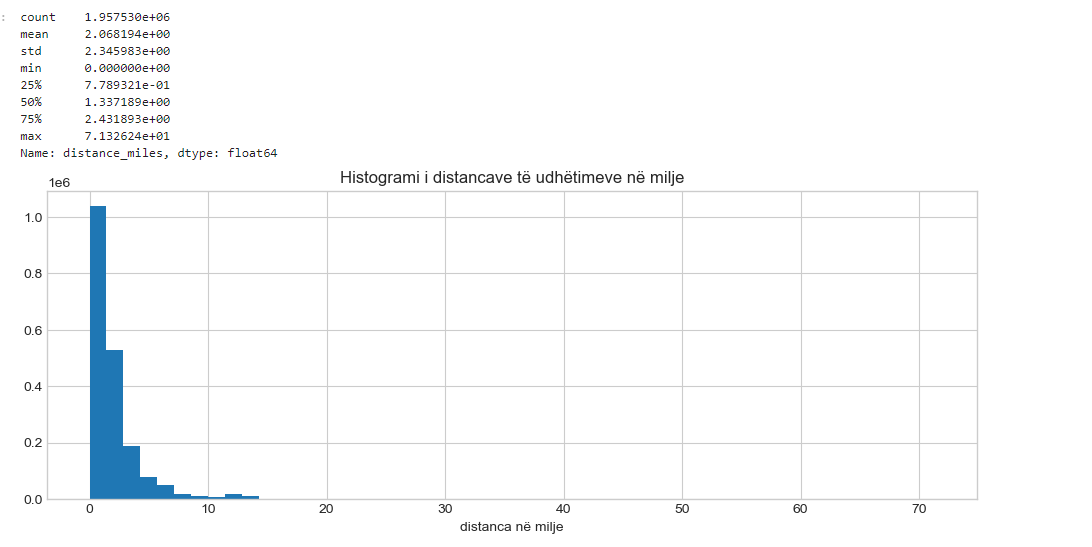
\includegraphics{./Figs/train21.png}
\end{frame}

\begin{frame}{Distanca dhe Çmimi}
\protect\hypertarget{distanca-dhe-uxe7mimi-4}{}
\begin{itemize}
\item
  Rezultatet e këtij operacioni tregojnë se shumica e udhëtimeve janë të
  shkurtra, me një kulm të vogël rreth \textasciitilde13 milje.
\item
  Ky kulm mund të jetë për shkak të udhëtimeve të aeroportit.
\end{itemize}
\end{frame}

\begin{frame}[fragile]{Numri i Pasagjerëve}
\protect\hypertarget{numri-i-pasagjeruxebve}{}
Të shohim gjithashtu ndikimin e numrit të pasagjerëve.

\AddToHookNext{env/Highlighting/begin}{\tiny}

\begin{Shaded}
\begin{Highlighting}[]
\CommentTok{\# Llogarisni mesataren e distancave dhe tarifave në varësi të numrit të pasagjerëve}
\NormalTok{df\_train.groupby(}\StringTok{\textquotesingle{}passenger\_count\textquotesingle{}}\NormalTok{)[[}\StringTok{\textquotesingle{}distance\_miles\textquotesingle{}}\NormalTok{, }\StringTok{\textquotesingle{}fare\_amount\textquotesingle{}}\NormalTok{]].mean()}
\end{Highlighting}
\end{Shaded}
\end{frame}

\begin{frame}{Numri i Pasagjerëve}
\protect\hypertarget{numri-i-pasagjeruxebve-1}{}
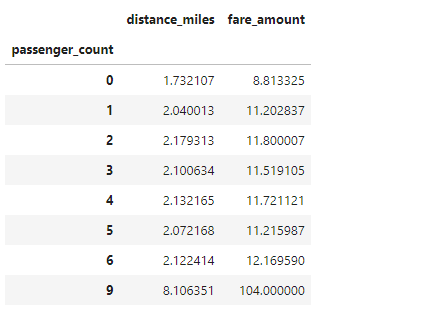
\includegraphics{./Figs/train22.png} \#\# Numri i Pasagjerëve

\begin{itemize}
\item
  Rezultati: Një numër pasagjerësh prej zero duket i çuditshëm.
\item
  Ndoshta një taksi që transporton disa mallra ose një gabim
  administrativ?
\end{itemize}
\end{frame}

\begin{frame}[fragile]{Tarifa për Milje}
\protect\hypertarget{tarifa-puxebr-milje}{}
Në vend që të shohim \textbf{fare\_amount}, përdorimi i `fare per mile'
gjithashtu ofron disa njohuri.

\AddToHookNext{env/Highlighting/begin}{\tiny}

\begin{Shaded}
\begin{Highlighting}[]
\CommentTok{\# Llogaritni mesataren e USD për milje}
\BuiltInTok{print}\NormalTok{(}\StringTok{"Mesatarja USD/Mile : }\SpecialCharTok{\{:0.2f\}}\StringTok{"}\NormalTok{.}\BuiltInTok{format}\NormalTok{(df\_train.fare\_amount.}\BuiltInTok{sum}\NormalTok{()}\OperatorTok{/}\NormalTok{df\_train.distance\_miles.}\BuiltInTok{sum}\NormalTok{()))}
\end{Highlighting}
\end{Shaded}


\includegraphics{./Figs/train23.png}
\end{frame}

\begin{frame}[fragile]{Grafiku i Pikave për Distancën dhe Tarifën}
\protect\hypertarget{grafiku-i-pikave-puxebr-distancuxebn-dhe-tarifuxebn}{}
\AddToHookNext{env/Highlighting/begin}{\tiny}

\begin{Shaded}
\begin{Highlighting}[]
\CommentTok{\# Trego grafikun e pikave për distancën dhe tarifën}
\NormalTok{fig, axs }\OperatorTok{=}\NormalTok{ plt.subplots(}\DecValTok{1}\NormalTok{, }\DecValTok{2}\NormalTok{, figsize}\OperatorTok{=}\NormalTok{(}\DecValTok{16}\NormalTok{,}\DecValTok{6}\NormalTok{))}
\NormalTok{axs[}\DecValTok{0}\NormalTok{].scatter(df\_train.distance\_miles, df\_train.fare\_amount, alpha}\OperatorTok{=}\FloatTok{0.2}\NormalTok{)}
\NormalTok{axs[}\DecValTok{0}\NormalTok{].set\_xlabel(}\StringTok{\textquotesingle{}distanca në milje\textquotesingle{}}\NormalTok{)}
\NormalTok{axs[}\DecValTok{0}\NormalTok{].set\_ylabel(}\StringTok{\textquotesingle{}tarifa USD\textquotesingle{}}\NormalTok{)}
\NormalTok{axs[}\DecValTok{0}\NormalTok{].set\_title(}\StringTok{\textquotesingle{}Të gjitha të dhënat\textquotesingle{}}\NormalTok{)}
\end{Highlighting}
\end{Shaded}
\end{frame}

\begin{frame}[fragile]{Grafiku i Pikave për Distancën dhe Tarifën
(vazhdim)}
\protect\hypertarget{grafiku-i-pikave-puxebr-distancuxebn-dhe-tarifuxebn-vazhdim}{}
\AddToHookNext{env/Highlighting/begin}{\tiny}

\begin{Shaded}
\begin{Highlighting}[]
\CommentTok{\# Trego një pamje të të dhënave të filtruara}
\NormalTok{idx }\OperatorTok{=}\NormalTok{ (df\_train.distance\_miles }\OperatorTok{\textless{}} \DecValTok{15}\NormalTok{) }\OperatorTok{\&}\NormalTok{ (df\_train.fare\_amount }\OperatorTok{\textless{}} \DecValTok{100}\NormalTok{)}
\NormalTok{axs[}\DecValTok{1}\NormalTok{].scatter(df\_train[idx].distance\_miles, df\_train[idx].fare\_amount, alpha}\OperatorTok{=}\FloatTok{0.2}\NormalTok{)}
\NormalTok{axs[}\DecValTok{1}\NormalTok{].set\_xlabel(}\StringTok{\textquotesingle{}distanca në milje\textquotesingle{}}\NormalTok{)}
\NormalTok{axs[}\DecValTok{1}\NormalTok{].set\_ylabel(}\StringTok{\textquotesingle{}tarifa USD\textquotesingle{}}\NormalTok{)}
\NormalTok{axs[}\DecValTok{1}\NormalTok{].set\_title(}\StringTok{\textquotesingle{}Pjesë e të dhënave me distancë \textless{} 15 milje, tarifë \textless{} $100\textquotesingle{}}\NormalTok{)}
\end{Highlighting}
\end{Shaded}
\end{frame}

\begin{frame}{Grafiku i Pikave për Distancën dhe Tarifën}
\protect\hypertarget{grafiku-i-pikave-puxebr-distancuxebn-dhe-tarifuxebn-1}{}
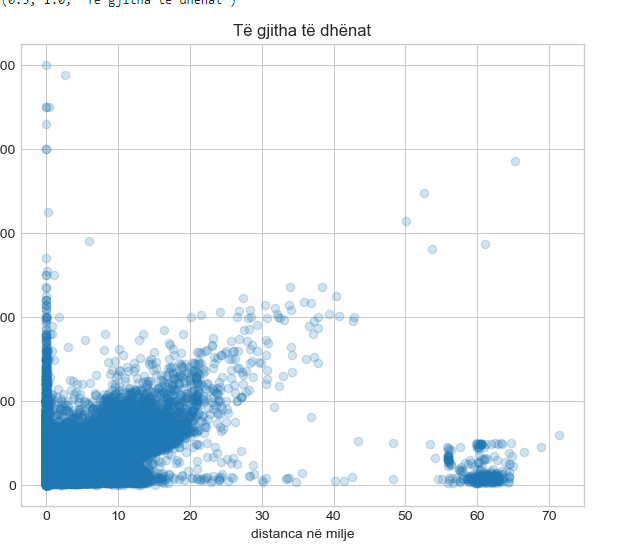
\includegraphics{./Figs/train24.png}
\end{frame}

\begin{frame}{Grafiku i Pikave për Distancën dhe Tarifën (vazhdim)}
\protect\hypertarget{grafiku-i-pikave-puxebr-distancuxebn-dhe-tarifuxebn-vazhdim-1}{}
Nga ky grafik vërejmë se:

\begin{itemize}
\item
  Ka udhëtime me distancë zero, por me një tarifë jo zero.
\item
  Ka disa udhëtime me \textgreater50 milje distancë udhëtimi por tarifë
  të ulët.
\item
  Linjat horizontale në grafikun e djathtë mund të tregojnë përsëri
  udhëtimet me tarifë fikse.
\end{itemize}
\end{frame}

\begin{frame}{Informacione mbi Tarifat e Taksive}
\protect\hypertarget{informacione-mbi-tarifat-e-taksive}{}
Kur kërkojmë për çmimet e taksive në NYC në Google, gjejmë:

\begin{itemize}
\item
  \$4.00 -- \$10.00 për një udhëtim prej 3 km.
\item
  Fillimi varion nga \$2.50 - \$3.30.
\end{itemize}
\end{frame}

\begin{frame}{Informacione mbi Tarifat e Taksive}
\protect\hypertarget{informacione-mbi-tarifat-e-taksive-1}{}
\begin{itemize}
\item
  Tarifa fillestare për shumicën e udhëtimeve (me përjashtim të JFK dhe
  aeroporteve të tjera) është 2,50 dollarë pas hyrjes.
\item
  Pas kësaj ka 0,5 dollarë çdo njësi ku njësia përcaktohet si 1/5 e
  miljes ose kur taksi po udhëton 12 milje në orë ose më shumë.
\end{itemize}
\end{frame}

\begin{frame}{Informacione mbi Tarifat e Taksive}
\protect\hypertarget{informacione-mbi-tarifat-e-taksive-2}{}
\begin{itemize}
\item
  0,5 dollarë shtesë shtesë midis orës 20:00 - 06:00.
\item
  Tarifa shtesë për orët e pikut të javës prej 1 dollarë e hënë-e premte
  nga ora 16:00-20:00.
\item
  Ka një shtesë prej 0,5 dollarësh MTA për të gjitha udhëtimet që
  përfundojnë në qarqet e Nju Jorkut ose Nassau, Suffolk, Westchester,
  Rockland, Dutchess, Orange ose Putnam.
\end{itemize}
\end{frame}

\begin{frame}{Informacione mbi Tarifat e Taksive}
\protect\hypertarget{informacione-mbi-tarifat-e-taksive-3}{}
\begin{itemize}
\tightlist
\item
  Ka një shtesë prej 0,3 dollarësh për përmirësim
\end{itemize}
\end{frame}

\begin{frame}[fragile]{Informacione mbi Tarifat e Taksive}
\protect\hypertarget{informacione-mbi-tarifat-e-taksive-4}{}
\AddToHookNext{env/Highlighting/begin}{\tiny}

\begin{Shaded}
\begin{Highlighting}[]
\CommentTok{\# hiqni pikat e të dhënave me distancë \textless{}0.05 milje}
\NormalTok{idx }\OperatorTok{=}\NormalTok{ (df\_train.distance\_miles }\OperatorTok{\textgreater{}=} \FloatTok{0.05}\NormalTok{)}
\BuiltInTok{print}\NormalTok{(}\StringTok{\textquotesingle{}Madhësia e vjetër: }\SpecialCharTok{\%d}\StringTok{\textquotesingle{}} \OperatorTok{\%} \BuiltInTok{len}\NormalTok{(df\_train))}
\NormalTok{df\_train }\OperatorTok{=}\NormalTok{ df\_train[idx]}
\BuiltInTok{print}\NormalTok{(}\StringTok{\textquotesingle{}Madhësia e re: }\SpecialCharTok{\%d}\StringTok{\textquotesingle{}} \OperatorTok{\%} \BuiltInTok{len}\NormalTok{(df\_train))}
\end{Highlighting}
\end{Shaded}
\end{frame}

\begin{frame}{Informacione mbi Tarifat e Taksive}
\protect\hypertarget{informacione-mbi-tarifat-e-taksive-5}{}
Kjo pastron të dhënat dhe bën analizën më të besueshme.

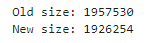
\includegraphics{./Figs/train25.png}
\end{frame}

\begin{frame}{Udhëtime me Tarifa Fikse}
\protect\hypertarget{udhuxebtime-me-tarifa-fikse}{}
\begin{itemize}
\item
  Disa udhëtime, si ato drejt/nga aeroporti, kanë tarifa fikse.
\item
  Një mënyrë për të eksploruar të dhënat është duke kontrolluar
  udhëtimet drejt/nga vende të njohura.
\item
  P.sh., një udhëtim drejt Aeroportit JFK, që shpesh ka çmim të fiksuar
  në varësi të distancës.
\end{itemize}
\end{frame}

\begin{frame}[fragile]{Koordinatat e Aeroportit JFK}
\protect\hypertarget{koordinatat-e-aeroportit-jfk}{}
\AddToHookNext{env/Highlighting/begin}{\tiny}

\begin{Shaded}
\begin{Highlighting}[]
\NormalTok{jfk }\OperatorTok{\textless{}{-}}\NormalTok{ c(}\OperatorTok{{-}}\FloatTok{73.7822222222}\NormalTok{, }\FloatTok{40.6441666667}\NormalTok{)}
\NormalTok{nyc }\OperatorTok{\textless{}{-}}\NormalTok{ c(}\OperatorTok{{-}}\FloatTok{74.0063889}\NormalTok{, }\FloatTok{40.7141667}\NormalTok{)}
\end{Highlighting}
\end{Shaded}
\end{frame}

\begin{frame}[fragile]{Funksioni për të Vizualizuar Tarifën pranë
Aeroportit}
\protect\hypertarget{funksioni-puxebr-tuxeb-vizualizuar-tarifuxebn-pranuxeb-aeroportit}{}
\AddToHookNext{env/Highlighting/begin}{\tiny}

\begin{Shaded}
\begin{Highlighting}[]
\KeywordTok{def}\NormalTok{ plot\_location\_fare(loc, name, }\BuiltInTok{range}\OperatorTok{=}\FloatTok{1.5}\NormalTok{):}
     \CommentTok{\# Zgjedh të gjitha pikë të dhënave me vendin e ngritjes brenda rrezes së aeroportit}
\NormalTok{    fig, axs }\OperatorTok{=}\NormalTok{ plt.subplots(}\DecValTok{1}\NormalTok{, }\DecValTok{2}\NormalTok{, figsize}\OperatorTok{=}\NormalTok{(}\DecValTok{14}\NormalTok{, }\DecValTok{5}\NormalTok{))}
\NormalTok{    idx }\OperatorTok{=}\NormalTok{ (distance(df\_train.pickup\_latitude, df\_train.pickup\_longitude, loc[}\DecValTok{1}\NormalTok{], loc[}\DecValTok{0}\NormalTok{]) }\OperatorTok{\textless{}} \BuiltInTok{range}\NormalTok{)}
\NormalTok{    df\_train[idx].fare\_amount.hist(bins}\OperatorTok{=}\DecValTok{100}\NormalTok{, ax}\OperatorTok{=}\NormalTok{axs[}\DecValTok{0}\NormalTok{])}
\NormalTok{    axs[}\DecValTok{0}\NormalTok{].set\_xlabel(}\StringTok{\textquotesingle{}Tarifa USD\textquotesingle{}}\NormalTok{)}
\NormalTok{    axs[}\DecValTok{0}\NormalTok{].set\_title(}\StringTok{\textquotesingle{}Histogram vendi i marrjes brenda }\SpecialCharTok{\{\}}\StringTok{ miles of }\SpecialCharTok{\{\}}\StringTok{\textquotesingle{}}\NormalTok{.}\BuiltInTok{format}\NormalTok{(}\BuiltInTok{range}\NormalTok{, name))}

\NormalTok{    idx }\OperatorTok{=}\NormalTok{ (distance(df\_train.dropoff\_latitude, df\_train.dropoff\_longitude, loc[}\DecValTok{1}\NormalTok{], loc[}\DecValTok{0}\NormalTok{]) }\OperatorTok{\textless{}} \BuiltInTok{range}\NormalTok{)}
\NormalTok{    df\_train[idx].fare\_amount.hist(bins}\OperatorTok{=}\DecValTok{100}\NormalTok{, ax}\OperatorTok{=}\NormalTok{axs[}\DecValTok{1}\NormalTok{])}
\NormalTok{    axs[}\DecValTok{1}\NormalTok{].set\_xlabel(}\StringTok{\textquotesingle{}Tarifa USD\textquotesingle{}}\NormalTok{)}
\NormalTok{    axs[}\DecValTok{1}\NormalTok{].set\_title(}\StringTok{\textquotesingle{}Histogram vendi i mbrritjes brenda }\SpecialCharTok{\{\}}\StringTok{ miles of }\SpecialCharTok{\{\}}\StringTok{\textquotesingle{}}\NormalTok{.}\BuiltInTok{format}\NormalTok{(}\BuiltInTok{range}\NormalTok{, name))}\OperatorTok{;}
\end{Highlighting}
\end{Shaded}
\end{frame}

\begin{frame}[fragile]{Vizualizoni Tarifën për JFK}
\protect\hypertarget{vizualizoni-tarifuxebn-puxebr-jfk}{}
\AddToHookNext{env/Highlighting/begin}{\tiny}

\begin{Shaded}
\begin{Highlighting}[]
\NormalTok{plot\_location\_fare(jfk, }\StringTok{\textquotesingle{}Aeroporti JFK\textquotesingle{}}\NormalTok{)}
\end{Highlighting}
\end{Shaded}
\end{frame}

\begin{frame}{Vizualizoni Tarifën për JFK}
\protect\hypertarget{vizualizoni-tarifuxebn-puxebr-jfk-1}{}
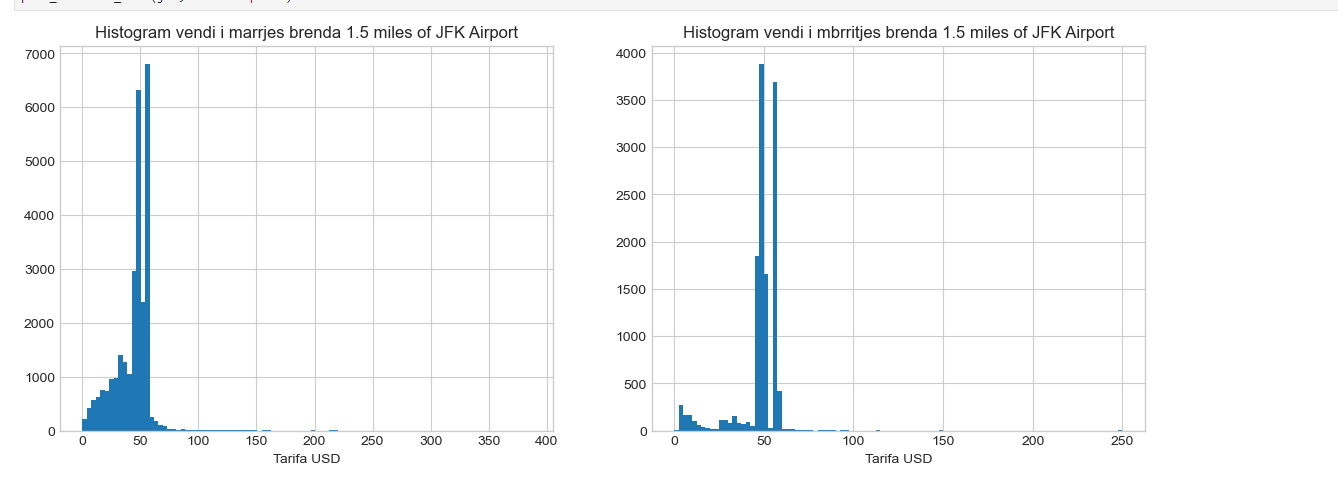
\includegraphics{./Figs/train26.png}
\end{frame}

\begin{frame}[fragile]{Aeroporte të Tjera}
\protect\hypertarget{aeroporte-tuxeb-tjera}{}
Po përsërisim analizën për aeroportet e tjera të NYC:

\AddToHookNext{env/Highlighting/begin}{\tiny}

\begin{Shaded}
\begin{Highlighting}[]
\NormalTok{ewr }\OperatorTok{=}\NormalTok{ (}\OperatorTok{{-}}\FloatTok{74.175}\NormalTok{, }\FloatTok{40.69}\NormalTok{) }\CommentTok{\# Aeroporti Newark}
\NormalTok{lgr }\OperatorTok{=}\NormalTok{ (}\OperatorTok{{-}}\FloatTok{73.87}\NormalTok{, }\FloatTok{40.77}\NormalTok{) }\CommentTok{\# Aeroporti LaGuardia}

\NormalTok{plot\_location\_fare(ewr, }\StringTok{\textquotesingle{}Aeroporti Newark\textquotesingle{}}\NormalTok{)}
\NormalTok{plot\_location\_fare(lgr, }\StringTok{\textquotesingle{}Aeroporti LaGuardia\textquotesingle{}}\NormalTok{)}
\end{Highlighting}
\end{Shaded}
\end{frame}

\begin{frame}{Aeroporte të Tjera}
\protect\hypertarget{aeroporte-tuxeb-tjera-1}{}
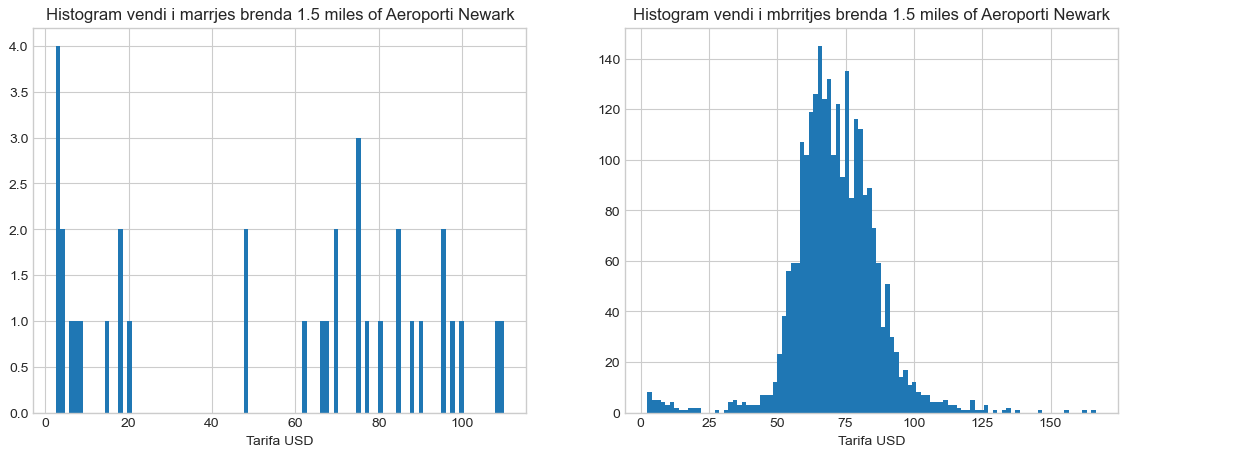
\includegraphics{./Figs/train27.png}
\end{frame}

\begin{frame}[fragile]{Tarifat Ndryshojnë Natën Krahasuar me Ditën}
\protect\hypertarget{tarifat-ndryshojnuxeb-natuxebn-krahasuar-me-dituxebn}{}
Për të parë lidhjen mes kohës dhe tarifës/km, shtojmë tre kolona të reja
në të dhëna: vitin, orën e ditës dhe tarifën USD për KM.

\AddToHookNext{env/Highlighting/begin}{\tiny}

\begin{Shaded}
\begin{Highlighting}[]
\NormalTok{df\_train[}\StringTok{\textquotesingle{}fare\_per\_mile\textquotesingle{}}\NormalTok{] }\OperatorTok{=}\NormalTok{ df\_train.fare\_amount }\OperatorTok{/}\NormalTok{ df\_train.distance\_miles}
\NormalTok{df\_train.fare\_per\_mile.describe()}
\end{Highlighting}
\end{Shaded}
\end{frame}

\begin{frame}{Tarifat Ndryshojnë Natën Krahasuar me Ditën}
\protect\hypertarget{tarifat-ndryshojnuxeb-natuxebn-krahasuar-me-dituxebn-1}{}
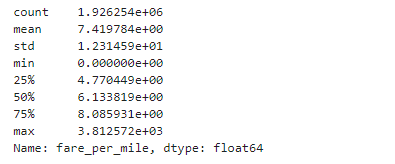
\includegraphics{./Figs/train28.png}
\end{frame}

\begin{frame}{Tarifat Ndryshojnë Natën Krahasuar me Ditën}
\protect\hypertarget{tarifat-ndryshojnuxeb-natuxebn-krahasuar-me-dituxebn-2}{}
\begin{itemize}
\item
  Tarifa maksimale USD/milje duket e lartë.
\item
  Kjo mund të jetë për shkak të të dhënave të gabuara të distancës ose
  tarifës.
\end{itemize}
\end{frame}

\begin{frame}{Tarifat Ndryshojnë Natën Krahasuar me Ditën}
\protect\hypertarget{tarifat-ndryshojnuxeb-natuxebn-krahasuar-me-dituxebn-3}{}
Tarifa e taksisë në përgjithësi llogaritet nga:

\[
y_{\text{tarifa}} = \theta_0 + \theta_1 \cdot x_{\text{distanca}} + \theta_2 \cdot x_{\text{koha}}
\]
\end{frame}

\begin{frame}{Tarifat Ndryshojnë Natën Krahasuar me Ditën}
\protect\hypertarget{tarifat-ndryshojnuxeb-natuxebn-krahasuar-me-dituxebn-4}{}
Për të shprehur tarifën për distancë:

\[
\frac{y_{\text{tarifa}}}{x_{\text{distanca}}} = \theta_0 \cdot x_{\text{distanca}} + \theta_1 + \theta_2 \cdot \frac{x_{\text{koha}}}{x_{\text{distanca}}}
\]
\end{frame}

\begin{frame}{Tarifat Ndryshojnë Natën Krahasuar me Ditën}
\protect\hypertarget{tarifat-ndryshojnuxeb-natuxebn-krahasuar-me-dituxebn-5}{}
Nëse supozojmë që për udhëtime më të shkurtra:

\[
x_{\text{distanca}} = c \cdot x_{\text{koha}}
\]

atëherë shprehet si:
\end{frame}

\begin{frame}{Tarifat Ndryshojnë Natën Krahasuar me Ditën}
\protect\hypertarget{tarifat-ndryshojnuxeb-natuxebn-krahasuar-me-dituxebn-6}{}
\[
\frac{y_{\text{tarifa}}}{x_{\text{distanca}}} = \theta_0 \cdot x_{\text{distanca}} + \theta'_1
\]

me:

\[
\theta'_1 = \theta_1 + \frac{\theta_2}{c}
\]
\end{frame}

\begin{frame}[fragile]{Tarifat Ndryshojnë Natën Krahasuar me Ditën}
\protect\hypertarget{tarifat-ndryshojnuxeb-natuxebn-krahasuar-me-dituxebn-7}{}
Në përfundim, tarifa për distancë është proporcionale me
1/distanca\_milje. Tani të vizatojmë grafikun.

\AddToHookNext{env/Highlighting/begin}{\tiny}

\begin{Shaded}
\begin{Highlighting}[]
\NormalTok{idx }\OperatorTok{=}\NormalTok{ (df\_train.distance\_miles }\OperatorTok{\textless{}} \DecValTok{3}\NormalTok{) }\OperatorTok{\&}\NormalTok{ (df\_train.fare\_amount }\OperatorTok{\textless{}} \DecValTok{100}\NormalTok{)}
\NormalTok{plt.scatter(df\_train[idx].distance\_miles, df\_train[idx].fare\_per\_mile)}
\NormalTok{plt.xlabel(}\StringTok{\textquotesingle{}Distanca milje\textquotesingle{}}\NormalTok{)}
\NormalTok{plt.ylabel(}\StringTok{\textquotesingle{}Tarifa për distancë milje\textquotesingle{}}\NormalTok{)}

\NormalTok{theta }\OperatorTok{=}\NormalTok{ (}\DecValTok{16}\NormalTok{, }\FloatTok{4.0}\NormalTok{)}
\NormalTok{x }\OperatorTok{=}\NormalTok{ np.linspace(}\FloatTok{0.1}\NormalTok{, }\DecValTok{3}\NormalTok{, }\DecValTok{50}\NormalTok{)}
\NormalTok{plt.plot(x, theta[}\DecValTok{0}\NormalTok{]}\OperatorTok{/}\NormalTok{x }\OperatorTok{+}\NormalTok{ theta[}\DecValTok{1}\NormalTok{], }\StringTok{\textquotesingle{}{-}{-}\textquotesingle{}}\NormalTok{, c}\OperatorTok{=}\StringTok{\textquotesingle{}r\textquotesingle{}}\NormalTok{, lw}\OperatorTok{=}\DecValTok{2}\NormalTok{)}\OperatorTok{;}
\end{Highlighting}
\end{Shaded}
\end{frame}

\begin{frame}{Tarifat Ndryshojnë Natën Krahasuar me Ditën}
\protect\hypertarget{tarifat-ndryshojnuxeb-natuxebn-krahasuar-me-dituxebn-8}{}
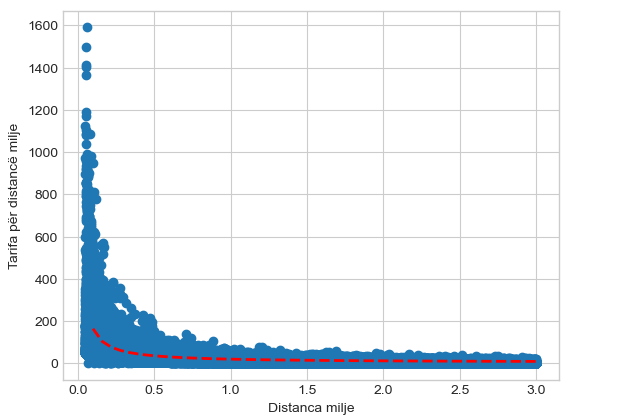
\includegraphics{./Figs/train29.png} \#\# Tarifat Ndryshojnë Natën
Krahasuar me Ditën

\begin{itemize}
\item
  Vini re se tarifa për distancë ka më shumë përhapje për distanca më të
  vogla (\textless0,5 milje) sesa distanca më të mëdha.
\item
  Kjo mund të shpjegohet si më poshtë: ne matim distancën nga pika në
  pikë dhe jo me rrugë.
\end{itemize}
\end{frame}

\begin{frame}{Tarifat Ndryshojnë Natën Krahasuar me Ditën}
\protect\hypertarget{tarifat-ndryshojnuxeb-natuxebn-krahasuar-me-dituxebn-9}{}
\begin{itemize}
\item
  Për distanca më të vogla, diferenca midis këtyre dy metodave të matjes
  pritet të jetë më e madhe.
\item
  Një arsye tjetër pse përhapja për distanca më të vogla është më e
  madhe mund të jetë për shkak të ngadalësimit të trafikut në orët e
  pikut.
\item
  Udhëtimet e shkurtra në orët e pikut ndryshojnë më shumë në
  kohëzgjatje.
\end{itemize}
\end{frame}

\begin{frame}{Tarifat Ndryshojnë Natën Krahasuar me Ditën}
\protect\hypertarget{tarifat-ndryshojnuxeb-natuxebn-krahasuar-me-dituxebn-10}{}
\begin{itemize}
\tightlist
\item
  Le të vazhdojmë me analizën e kohës dhe tarifës për distancë.
\end{itemize}
\end{frame}

\begin{frame}{Tarifat Ndryshojnë Natën Krahasuar me Ditën}
\protect\hypertarget{tarifat-ndryshojnuxeb-natuxebn-krahasuar-me-dituxebn-11}{}
\begin{itemize}
\tightlist
\item
  Dp përdorim një tabelë \textbf{pivot} panda për të bërë një
  përmbledhje dhe për t'i vizatuar ato.
\end{itemize}
\end{frame}

\begin{frame}[fragile]{Tarifat Ndryshojnë Natën Krahasuar me Ditën}
\protect\hypertarget{tarifat-ndryshojnuxeb-natuxebn-krahasuar-me-dituxebn-12}{}
\AddToHookNext{env/Highlighting/begin}{\tiny}

\begin{Shaded}
\begin{Highlighting}[]
\NormalTok{df\_train.pivot\_table(}\StringTok{\textquotesingle{}fare\_per\_mile\textquotesingle{}}\NormalTok{, index}\OperatorTok{=}\StringTok{\textquotesingle{}hour\textquotesingle{}}\NormalTok{, columns}\OperatorTok{=}\StringTok{\textquotesingle{}year\textquotesingle{}}\NormalTok{).plot(figsize}\OperatorTok{=}\NormalTok{(}\DecValTok{14}\NormalTok{,}\DecValTok{6}\NormalTok{))}
\NormalTok{plt.ylabel(}\StringTok{\textquotesingle{}Tarifa $USD / milje\textquotesingle{}}\NormalTok{)}\OperatorTok{;}
\end{Highlighting}
\end{Shaded}
\end{frame}

\begin{frame}{Tarifat Ndryshojnë Natën Krahasuar me Ditën}
\protect\hypertarget{tarifat-ndryshojnuxeb-natuxebn-krahasuar-me-dituxebn-13}{}
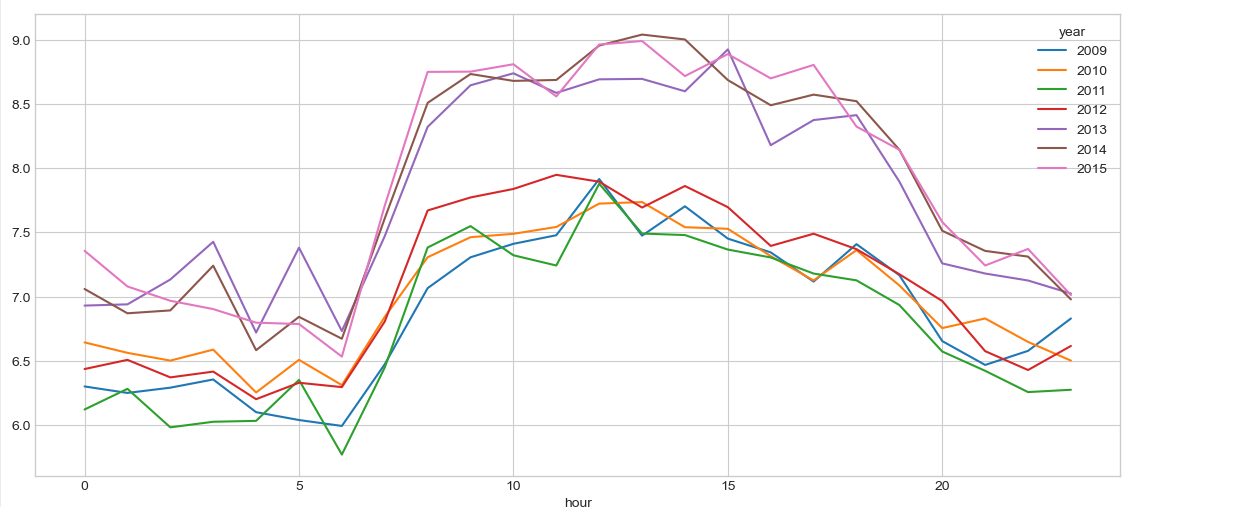
\includegraphics{./Figs/train30.png} \#\# Tarifat Ndryshojnë Natën
Krahasuar me Ditën

Mund të shihet qartë se tarifa \$USD/milje ndryshon me kalimin e viteve
dhe me kalimin e orëve.
\end{frame}

\begin{frame}{Tarifat Ndryshojnë Natën Krahasuar me Ditën}
\protect\hypertarget{tarifat-ndryshojnuxeb-natuxebn-krahasuar-me-dituxebn-14}{}
Për të hetuar më tej këtë, përdorim hartën e Google për të llogaritur
kohëzgjatjen e pritshme të dy udhëtimeve:

\begin{itemize}
\item
  Udhëtimi 1: nga Muzeu i Qytetit të Nju Jorkut në Teatrin Beacon, 4.5
  km, pa lënë Manhatten
\item
  Udhëtimi 2: nga Times Squared në Parkun Maria Hermandez, 12 km, duke
  lënë Times Squared nëpërmjet tunelit Queens Midtown (rruga me pagesë)
\end{itemize}
\end{frame}

\begin{frame}{Tarifat Ndryshojnë Natën Krahasuar me Ditën}
\protect\hypertarget{tarifat-ndryshojnuxeb-natuxebn-krahasuar-me-dituxebn-15}{}
\begin{itemize}
\item
  Sasia e trafikut përcakton kohëzgjatjen e udhëtimit dhe rrjedhimisht
  tarifën.
\item
  Ndërsa sasia e trafikut varet nga ora e ditës.
\end{itemize}
\end{frame}

\begin{frame}[fragile]{Tarifat Ndryshojnë Natën Krahasuar me Ditën}
\protect\hypertarget{tarifat-ndryshojnuxeb-natuxebn-krahasuar-me-dituxebn-16}{}
\AddToHookNext{env/Highlighting/begin}{\tiny}

\begin{Shaded}
\begin{Highlighting}[]
\NormalTok{hours }\OperatorTok{=}\NormalTok{ [}\DecValTok{0}\NormalTok{, }\DecValTok{1}\NormalTok{, }\DecValTok{2}\NormalTok{, }\DecValTok{3}\NormalTok{, }\DecValTok{4}\NormalTok{, }\DecValTok{5}\NormalTok{, }\DecValTok{6}\NormalTok{, }\DecValTok{7}\NormalTok{, }\DecValTok{8}\NormalTok{, }\DecValTok{9}\NormalTok{, }\DecValTok{10}\NormalTok{, }\DecValTok{11}\NormalTok{, }\DecValTok{12}\NormalTok{, }\OperatorTok{\textbackslash{}}
         \DecValTok{13}\NormalTok{, }\DecValTok{14}\NormalTok{, }\DecValTok{15}\NormalTok{, }\DecValTok{16}\NormalTok{, }\DecValTok{17}\NormalTok{, }\DecValTok{18}\NormalTok{, }\DecValTok{19}\NormalTok{, }\DecValTok{20}\NormalTok{, }\DecValTok{21}\NormalTok{, }\DecValTok{22}\NormalTok{, }\DecValTok{23}\NormalTok{]}

\CommentTok{\# kohëzgjatja minimale dhe maksimale në minuta}
\NormalTok{trip1\_min }\OperatorTok{=}\NormalTok{ [}\DecValTok{10}\NormalTok{, }\DecValTok{10}\NormalTok{, }\DecValTok{10}\NormalTok{, }\DecValTok{10}\NormalTok{, }\DecValTok{10}\NormalTok{, }\DecValTok{10}\NormalTok{, }\DecValTok{10}\NormalTok{, }\DecValTok{12}\NormalTok{, }\DecValTok{14}\NormalTok{, }\DecValTok{14}\NormalTok{, }\DecValTok{14}\NormalTok{, }\DecValTok{14}\NormalTok{, }\OperatorTok{\textbackslash{}}
             \DecValTok{14}\NormalTok{, }\DecValTok{14}\NormalTok{, }\DecValTok{14}\NormalTok{, }\DecValTok{14}\NormalTok{, }\DecValTok{14}\NormalTok{, }\DecValTok{12}\NormalTok{, }\DecValTok{12}\NormalTok{, }\DecValTok{12}\NormalTok{, }\DecValTok{12}\NormalTok{, }\DecValTok{12}\NormalTok{, }\DecValTok{10}\NormalTok{, }\DecValTok{10}\NormalTok{]}
\NormalTok{trip1\_max }\OperatorTok{=}\NormalTok{ [}\DecValTok{20}\NormalTok{, }\DecValTok{18}\NormalTok{, }\DecValTok{16}\NormalTok{, }\DecValTok{16}\NormalTok{, }\DecValTok{16}\NormalTok{, }\DecValTok{18}\NormalTok{, }\DecValTok{22}\NormalTok{, }\DecValTok{26}\NormalTok{, }\DecValTok{40}\NormalTok{, }\DecValTok{35}\NormalTok{, }\DecValTok{35}\NormalTok{, }\DecValTok{35}\NormalTok{, }\OperatorTok{\textbackslash{}}
             \DecValTok{35}\NormalTok{, }\DecValTok{35}\NormalTok{, }\DecValTok{35}\NormalTok{, }\DecValTok{40}\NormalTok{, }\DecValTok{35}\NormalTok{, }\DecValTok{30}\NormalTok{, }\DecValTok{28}\NormalTok{, }\DecValTok{28}\NormalTok{, }\DecValTok{26}\NormalTok{, }\DecValTok{26}\NormalTok{, }\DecValTok{24}\NormalTok{, }\DecValTok{24}\NormalTok{]}

\NormalTok{trip2\_min }\OperatorTok{=}\NormalTok{ [}\DecValTok{18}\NormalTok{, }\DecValTok{18}\NormalTok{, }\DecValTok{18}\NormalTok{, }\DecValTok{18}\NormalTok{, }\DecValTok{18}\NormalTok{, }\DecValTok{18}\NormalTok{, }\DecValTok{20}\NormalTok{, }\DecValTok{24}\NormalTok{, }\DecValTok{28}\NormalTok{, }\DecValTok{30}\NormalTok{, }\DecValTok{30}\NormalTok{, }\DecValTok{30}\NormalTok{, }\OperatorTok{\textbackslash{}}
             \DecValTok{28}\NormalTok{, }\DecValTok{28}\NormalTok{, }\DecValTok{26}\NormalTok{, }\DecValTok{28}\NormalTok{, }\DecValTok{30}\NormalTok{, }\DecValTok{28}\NormalTok{, }\DecValTok{26}\NormalTok{, }\DecValTok{22}\NormalTok{, }\DecValTok{22}\NormalTok{, }\DecValTok{22}\NormalTok{, }\DecValTok{20}\NormalTok{, }\DecValTok{20}\NormalTok{]}
\NormalTok{trip2\_max }\OperatorTok{=}\NormalTok{ [}\DecValTok{35}\NormalTok{, }\DecValTok{35}\NormalTok{, }\DecValTok{30}\NormalTok{, }\DecValTok{28}\NormalTok{, }\DecValTok{28}\NormalTok{, }\DecValTok{30}\NormalTok{, }\DecValTok{40}\NormalTok{, }\DecValTok{55}\NormalTok{, }\DecValTok{75}\NormalTok{, }\DecValTok{75}\NormalTok{, }\DecValTok{70}\NormalTok{, }\DecValTok{70}\NormalTok{, }\OperatorTok{\textbackslash{}}
             \DecValTok{60}\NormalTok{, }\DecValTok{60}\NormalTok{, }\DecValTok{60}\NormalTok{, }\DecValTok{60}\NormalTok{, }\DecValTok{60}\NormalTok{, }\DecValTok{65}\NormalTok{, }\DecValTok{55}\NormalTok{, }\DecValTok{45}\NormalTok{, }\DecValTok{45}\NormalTok{, }\DecValTok{50}\NormalTok{, }\DecValTok{45}\NormalTok{, }\DecValTok{40}\NormalTok{]}
\end{Highlighting}
\end{Shaded}
\end{frame}

\begin{frame}[fragile]{Tarifat Ndryshojnë Natën Krahasuar me Ditën
(vazhdim)}
\protect\hypertarget{tarifat-ndryshojnuxeb-natuxebn-krahasuar-me-dituxebn-vazhdim}{}
\AddToHookNext{env/Highlighting/begin}{\tiny}

\begin{Shaded}
\begin{Highlighting}[]
\CommentTok{\# Vizato grafikun e kohës së udhëtimit të vlerësuar për dy udhëtime duke përdorur informacionin e trafikut të Google Maps}
\NormalTok{plt.figure(figsize}\OperatorTok{=}\NormalTok{(}\DecValTok{12}\NormalTok{, }\DecValTok{5}\NormalTok{))}

\CommentTok{\# Vizato trip1 (2.7 milje) me kohën minimale dhe maksimale të udhëtimit}
\NormalTok{plt.plot(hours, trip1\_min, }\StringTok{\textquotesingle{}{-}{-}\textquotesingle{}}\NormalTok{, c}\OperatorTok{=}\StringTok{\textquotesingle{}b\textquotesingle{}}\NormalTok{, label}\OperatorTok{=}\StringTok{"trip1 (2.7 milje) {-} koha minimale"}\NormalTok{)}
\NormalTok{plt.plot(hours, trip1\_max, }\StringTok{\textquotesingle{}{-}\textquotesingle{}}\NormalTok{, c}\OperatorTok{=}\StringTok{\textquotesingle{}b\textquotesingle{}}\NormalTok{, label}\OperatorTok{=}\StringTok{"trip1 (2.7 milje) {-} koha maksimale"}\NormalTok{)}

\CommentTok{\# Vizato trip2 (7.2 milje) me kohën minimale dhe maksimale të udhëtimit}
\NormalTok{plt.plot(hours, trip2\_min, }\StringTok{\textquotesingle{}{-}{-}\textquotesingle{}}\NormalTok{, c}\OperatorTok{=}\StringTok{\textquotesingle{}r\textquotesingle{}}\NormalTok{, label}\OperatorTok{=}\StringTok{"trip2 (7.2 milje) {-} koha minimale"}\NormalTok{)}
\NormalTok{plt.plot(hours, trip2\_max, }\StringTok{\textquotesingle{}{-}\textquotesingle{}}\NormalTok{, c}\OperatorTok{=}\StringTok{\textquotesingle{}r\textquotesingle{}}\NormalTok{, label}\OperatorTok{=}\StringTok{"trip2 (7.2 milje) {-} koha maksimale"}\NormalTok{)}

\CommentTok{\# Vendos etiketën e boshtit x si \textquotesingle{}ora e ditës\textquotesingle{}}
\NormalTok{plt.xlabel(}\StringTok{\textquotesingle{}ora e ditës\textquotesingle{}}\NormalTok{)}

\CommentTok{\# Vendos etiketën e boshtit y si \textquotesingle{}koha e drejtimit (min)\textquotesingle{}}
\NormalTok{plt.ylabel(}\StringTok{\textquotesingle{}koha e drejtimit (min)\textquotesingle{}}\NormalTok{)}

\CommentTok{\# Vendos titullin e grafikut si \textquotesingle{}Koha e vlerësuar e drejtimit për dy udhëtime duke përdorur informacionin e trafikut të Google Maps\textquotesingle{}}
\NormalTok{plt.title(}\StringTok{\textquotesingle{}Koha e vlerësuar e drejtimit për dy udhëtime duke përdorur informacionin e trafikut të Google Maps\textquotesingle{}}\NormalTok{)}

\CommentTok{\# Shto një legjendë për të dalluar vizatimet}
\NormalTok{plt.legend()}
\end{Highlighting}
\end{Shaded}
\end{frame}

\begin{frame}{Tarifat Ndryshojnë Natën Krahasuar me Ditën}
\protect\hypertarget{tarifat-ndryshojnuxeb-natuxebn-krahasuar-me-dituxebn-17}{}
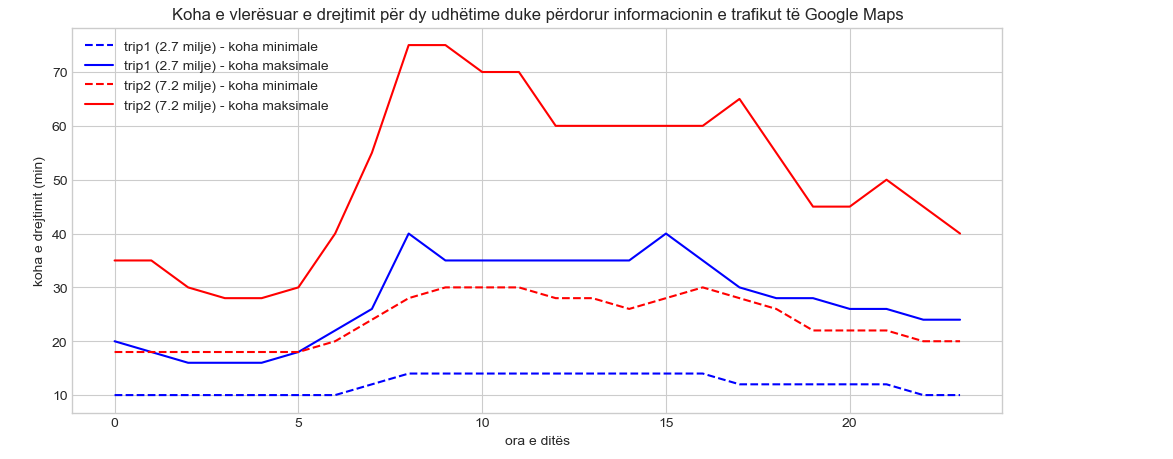
\includegraphics{./Figs/train31.png}
\end{frame}

\end{document}
